%!TEX program = pdflatex
% Author Alfredo Sánchez Alberca (asalber@ceu.es)

\documentclass[a4paper,titlepage]{article}
%===============================================
\usepackage[english]{babel}
\usepackage[utf8]{inputenc}
\usepackage[top=3cm, bottom=3cm, left=2.54cm, right=2.54cm, marginparwidth=2mm]{geometry}

% COLORS
\usepackage[table]{xcolor}
\definecolor{color1}{RGB}{5,161,230} % Light blue
\definecolor{color2}{RGB}{238,50,36} % Red
\definecolor{color3}{RGB}{0,205,0} % Light Green
\definecolor{ocre}{RGB}{243,102,25} % Define the orange color used for highlighting throughout the book
\definecolor{blueceu}{RGB}{5,161,230} % Blue color of CEU logo
\definecolor{greenceu}{RGB}{185,209,16} % Green color of CEU logo
\definecolor{redceu}{RGB}{238,50,36} % Red color of CEU logo
\definecolor{grayceu}{RGB}{111,107,83} % Gray color of CEU logo
\definecolor{chaptergrey}{RGB}{5,161,230} % Blue color of CEU logo

% MATH
\usepackage{amsmath}
\usepackage{amssymb}
\usepackage{amsthm}
\DeclareMathOperator{\sen}{sen}
\DeclareMathOperator{\arcsen}{arcsen}
\DeclareMathOperator{\tg}{tg}
\DeclareMathOperator{\arctg}{arctg}

% GRAPHICS
\usepackage{graphicx}
\usepackage{tikz}
\usepackage{pgfplots}

\usepackage{multicol}
\usepackage[inline]{enumitem}
\usepackage{fancyhdr}
\pagestyle{fancy}
\lhead{\textsc{\textcolor{blueceu}{CEU San Pablo University}}}
\rhead{\textsl{\textsf{\textcolor{blueceu}{Department of Applied Math and Statistics}}}}
\renewcommand{\headrulewidth}{0pt}

\usepackage{booktabs}


% SECTIONS
\usepackage{titlesec}
\titleformat*{\section}{\normalfont\Large\bfseries\color{color1}}


% % SOLUTIONS
% \newif\ifsolution
% % \solutiontrue  % Comment to hide solutions
%
% \newtheoremstyle{solution} % Theorem style name
% {-5pt} % Space above
% {7pt} % Space below
% {\normalfont} % Body font
% {-28pt} % Indent amount
% {\bf} % Theorem head font
% {\kern-11.5pt} % Punctuation after theorem head
% {19pt} % Space after theorem head
% {\begin{tikzpicture}
% \draw (0,0) node [fill=color2, xshift=4mm, inner
% sep=2pt]{\includegraphics[scale=0.3]{img/bulb}};
% \end{tikzpicture}}
%
% \theoremstyle{solution}
% \newtheorem{solutionT}{Solution}
%
% \RequirePackage[framemethod=default]{mdframed}
%
% % Solution box
% \newmdenv[skipabove=7pt,
% skipbelow=10pt,
% rightline=false,
% leftline=true,
% topline=false,
% bottomline=false,
% linecolor=color2,
% backgroundcolor=black!5,
% innerleftmargin=5pt,
% innerrightmargin=5pt,
% innertopmargin=4pt,
% innerbottommargin=5pt,
% leftmargin=0pt,
% rightmargin=0pt,
% linewidth=4pt]{solBox}
%
% \usepackage{comment}
% \ifsolution
%   \newenvironment{sol}{\ifsolution\begin{solBox}\begin{solutionT}}{\end{solutionT}\end{solBox}\fi}
% \else
%   \excludecomment{sol}
% \fi

% PDF
\usepackage[colorlinks=true]{hyperref}
\hypersetup{pdfauthor={Alfredo Sánchez Alberca (asalber@ceu.es)}, pdftitle={Calculus problems} }
\usepackage{url}

\renewcommand{\floatpagefraction}{.8}
\renewcommand{\textfraction}{.1}

% SOLUTIONS SETTINGS
\usepackage{probsoln-alf}
\reversemarginpar
\showshortanswers
%\showanswers
%\PSNrandseed{2007}

\begin{document}
\sloppy

\title{\vskip 2cm
\Huge \textbf{\textsf{\quad \textcolor{blueceu}{CALCULUS PROBLEMS}\quad}}\\
   \vskip 1cm
\Large \sffamily
\begin{tabular}{rl}
\textcolor{blueceu}{Subject:} & Mathematics\\
\textcolor{blueceu}{Course:} & $1^{st}$\\
\textcolor{blueceu}{Degree:} &  Pharmacy\\
\textcolor{blueceu}{Year:} & 2016-2017\\
\textcolor{blueceu}{Authors:} & Pablo Ares Gastesi (\url{pablo.aresgastesi@ceu.es})\\
& Eduardo L\'opez Ram\'irez (\url{elopez@ceu.es})\\
& Anselmo Romero Lim\'on (\url{arlimon@ceu.es})\\
& Alfredo S\'anchez Alberca (\url{asalber@ceu.es})
\end{tabular}
}

\author{}
\date{
\includegraphics[scale=0.3]{img/logo_uspceu_01}}

\maketitle
\newpage
\tableofcontents
\newpage

% Autor: Alfredo Sánchez Alberca (asalber@ceu.es)

\newproblem{der-1}{gen}{}
%ENUNCIADO
{Estudiar si es derivable la función $f(x)=\sqrt[3]{x-1}$ en el punto $x=1$.
}
%SOLUCIÓN
{La función no es derivable ya que $f'(1)=\lim_{h\rightarrow 0}\frac{f(1+h)-f(1)}{h} = \infty$.
}
%RESOLUCIÓN
{Aplicando la definición de derivada, tenemos:
\begin{align*}
f'(1) = \lim_{h\rightarrow 0}\frac{f(1+h)-f(1)}{h} = \lim_{h\rightarrow 0}\frac{\sqrt[3]{1+h-1}-\sqrt[3]{1-1}}{h} = \lim_{h\rightarrow 0}\frac{\sqrt[3]{h}}{h} = \lim_{h\rightarrow 0} h^{-2/3} = \infty.
\end{align*}
Así pues, la función no es derivable en $x=1$.
}


\newproblem*{der-2}{gen}{}
%ENUNCIADO
{Comprobar que la función $f(x)=|x-1|$ es continua en $x=1$ pero no es derivable en dicho punto.
}


\newproblem*{der-3}{gen}{}
%ENUNCIADO
{Estudiar la derivabilidad de $f$ en los puntos $x=-1$, $x=2$ y $x=3$ siendo
\[ f(x)=
\begin{cases}
\log(-x) & \mbox{si $x<-1$,} \\
\sen \pi x & \mbox{si $x\in [-1,2]$,} \\
x/2 & \mbox{si $x\in (2,3)$,} \\
3/2 & \mbox{si $x\geq 3$.}
\end{cases}
\]
}


\newproblem*{der-4}{gen}{}
%ENUNCIADO
{Estudiar la derivabilidad y calcular la derivada, donde exista, de la función
\[ f(x)=
\begin{cases}
(x+3)^2 & \mbox{si $x\leq -2$,} \\
x^2-3 & \mbox{si $-2\leq x\leq -1$,} \\
0 & \mbox{si $-1< x <0$,} \\
x^2 & \mbox{si $0\leq x \leq 1$,} \\
\cos \dfrac{1}{x-1} & \mbox{si $1< x\leq 2$,} \\
2x-3 & \mbox{si $x>2$.}
\end{cases}
\]
}


\newproblem*{der-5}{gen}{}
%ENUNCIADO
{Probar que no es derivable en $x=0$ la siguiente función:
\[ f(x)=
\begin{cases}
e^x-1 & \mbox{si $x\geq 0$,}  \\
x^3 & \mbox{si $x<0$.}
\end{cases}
\]
}


\newproblem{der-6}{gen}{}
%ENUNCIADO
{Estudiar la derivabilidad de las siguientes funciones y hallar la función derivada correspondiente en los puntos donde exista.
\begin{enumerate}
\item  $f(x)=
\begin{cases}
1-x & \mbox{si $x\leq 0$,} \\
e^{-x} & \mbox{si $x>0$.}
\end{cases}
$
\item  $g(x)=2x+|x^2-2|$.
\end{enumerate}
}
%SOLUCIÓN
{\begin{enumerate}
\item La función es derivable en $x=0$ ya que $f'^-(0)=f'^+(0) = 1$ y la derivada es
\[f'(x)=
\begin{cases}
-1 & \mbox{si $x\leq 0$,} \\
-e^{-x} & \mbox{si $x>0$.}
\end{cases}
\]
\item La función no es derivable en $x=-\sqrt{2}$ ya que $g'^-(-\sqrt{2})=2-2\sqrt 2$ y $g'^+(-\sqrt{2})=2+2\sqrt 2$, y tampoco es derivable en $x=\sqrt 2$ ya que $x=-\sqrt{2}$ ya que $g'^-(\sqrt{2})=2-2\sqrt 2$ y $g'^+(\sqrt{2})=2+2\sqrt 2$. En el resto de los puntos, la derivada vale
\[
g'(x)=
\begin{cases}
2+2x & \mbox{si $x< -\sqrt{2}$,} \\
2-2x & \mbox{si $-\sqrt 2 < x < \sqrt 2$,}\\
2+2x & \mbox{si $x > \sqrt 2$.}
\end{cases}
\]
\end{enumerate}
}
%RESOLUCIÓN
{Para estudiar la derivabilidad primero vamos a expresar la función $|x^2-2|$ como una función a trozos. Para ello necesitamos saber en qué puntos la función $x^2-2$ es positiva, y en qué puntos es negativa. Si calculamos las raíces de esta función tenemos:
\[
|x^2-2| = 0 \Leftrightarrow x^2 = 2 \Leftrightarrow x = \pm \sqrt 2.
\]
Si estudiamos el signo en los intervalos definidos por las raíces, podemos comprobar fácilmente sin más que calcular la función en cualquier punto de los intervalos que $x^2-2$ es negativa en el intervalo $(-\sqrt 2, \sqrt 2)$ y positiva en el resto de su dominio.
Por tanto, podemos expresar el valor absoluto de la siguiente manera:
\[
|x^2-2| =
\begin{cases}
x^2-2 & \mbox{si $x< -\sqrt{2}$,} \\
-x^2+2 & \mbox{si $-\sqrt 2 \leq x \leq \sqrt 2$,}\\
x^2-2 & \mbox{si $x > \sqrt 2$.}
\end{cases}
\]
y entonces, la función original puede expresarse como:
\[
g(x) =
\begin{cases}
2x+x^2-2 & \mbox{si $x< -\sqrt{2}$,} \\
2x-x^2+2 & \mbox{si $-\sqrt 2 \leq x \leq \sqrt 2$,}\\
2x+x^2-2 & \mbox{si $x > \sqrt 2$.}
\end{cases}
\]
Ahora, si estudiamos la derivabilidad de cada una de estas funciones en los trozos correspondientes, vemos que ambas son polinomios y por tanto son derivables en sus dominios. Faltaría por estudiar la derivabilidad en los puntos donde cambia la definición de la función. Para ello hay que estudiar la derivada por la izquierda y por la derecha y ver si coinciden. En el punto $x=-\sqrt 2$ tenemos:

\begin{align*}
g'^-(-\sqrt{2}) &= 2-2\sqrt 2\\
g'^+(-\sqrt{2}) &= 2+2\sqrt 2
\end{align*}

Y como ámbas derivadas no coinciden la función no es derivable en $x=-\sqrt 2$. En $x=\sqrt 2 $ tenemos:

\begin{align*}
g'^-(\sqrt{2}) &= 2-2\sqrt 2\\
g'^+(\sqrt{2}) &= 2+2\sqrt 2
\end{align*}

Ambas derivadas no coinciden y tampoco es derivable en $x=\sqrt 2$.

Así pues, la derivada vale:
\[
g'(x)=
\begin{cases}
2+2x & \mbox{si $x< -\sqrt{2}$,} \\
2-2x & \mbox{si $-\sqrt 2 < x < \sqrt 2$,}\\
2+2x & \mbox{si $x > \sqrt 2$.}
\end{cases}
\]
}


\newproblem{der-7}{gen}{}
%ENUNCIADO
{Dada la función
\[ f(x)=
\begin{cases}
ax+\dfrac{1}{x} & \mbox{si $x\leq -1$,} \\
x^2+bx & \mbox{si $-1<x\leq 1$,} \\
\log (x^2) & \mbox{si $x>1$.}
\end{cases}
\]
donde $a$ y $b$ son constantes.
\begin{enumerate}
\item  ¿Existen algunos valores de las constantes para los que la función sea continua en todo su dominio? En caso afirmativo, indicar cuáles son esos valores, y en caso contrario, razonar la respuesta.
\item  ¿Existen algunos valores de las constantes para los que la función sea derivable en todo su dominio? En caso afirmativo, indicar cuáles son esos valores, y en caso contrario, razonar la respuesta.
\end{enumerate}
}
%SOLUCIÓN
{\begin{enumerate}
\item La función es continua en todo el dominio si $a=-3$ y $b=-1$.
\item No existe ningún valor de $a$ y $b$ con los que la función sea derivable en todo el dominio.
\end{enumerate}
}
%RESOLUCIÓN
{
}


\newproblem{der-8}{gen}{*}
%ENUNCIADO
{Dada la función
\[
f(x)=
\begin{cases}
\sen^2x & \mbox{si $x\leq 0$},  \\
ax^2+b &  \mbox{si $0<x\leq c$},  \\
\ln x &  \mbox{si $c<x$},
\end{cases}
\]
con $a$, $b$ y $c$ constantes, ¿existe algún valor de las constantes de manera que la función sea continua y derivable en todo su dominio?
}
%SOLUCIÓN
{$a=\frac{1}{2e}, b=0, c=e^{1/2}.$
}
%RESOLUCIÓN
{Estudiaremos primero la continuidad y luego la derivabilidad.

Las funciones $\sen 2x$, $ax^2+b$ y $\ln x$ son todas contínuas en sus dominios, por tanto, basta con estudiar los puntos donde cambia la definici\'{o}n de la funci\'{o}n.

En el punto $x=0$ tenemos:
\begin{align*}
\lim_{x\rightarrow 0^{-}}f(x) &= \lim_{x\rightarrow 0^{-}}\sen^2x=\sen^20=0, \\
\lim_{x\rightarrow 0^{+}}f(x) &= \lim_{x\rightarrow 0^{+}}ax^2+b=a0^2+b=b, \\
f(0) &= \sen^20=0.
\end{align*}

Luego la función será contínua en $x=0$ si y sólo si $b=0$.

En el punto $x=c$ tenemos:
\begin{align*}
\lim_{x\rightarrow c^{-}}f(x) &= \lim_{x\rightarrow c^{-}}ax^2+b=ac^2+b, \\
\lim_{x\rightarrow c^{+}}f(x) &= \lim_{x\rightarrow c^{+}}\ln x=\ln c, \\
f(c) &= ac^2+b.
\end{align*}

Luego la función será contínua en $x=c$ si y sólo si $ac^2+b=\ln c$.

Por consiguiente, para que la función sea contínua en todo su dominio deben cumplirse las dos ecuaciones siguientes:
\[
\begin{cases}
b=0 \\
ac^2+b = \ln c
\end{cases}
\]

Con la derivabilidad ocurre lo mismo pues las funciones $\sen 2x$ , $ax^2+b$ y $\ln x$ son derivables en su dominio y basta con estudiar la existencia de la derivada en los puntos donde cambia la definición de la función.

En el punto $x=0$ (imponemos $b=0$ pues de lo contrario la función no sería continua en este punto y tampoco derivable) tenemos:
\begin{align*}
\lim_{h\rightarrow 0^{-}}\frac{f(0+h)-f(0)}{h} &= \lim_{h\rightarrow 0^{-}}\frac{\sen^2(0+h)-\sen^20}{h} = \lim_{h\rightarrow 0^{-}}\frac{\sen^2h}{h}\stackrel{\text{L}^{\prime }\text{H\^{o}pital}}{=}\lim_{h\rightarrow 0^{-}}\frac{2\sen h\cos h}{1}=0, \\
\lim_{h\rightarrow 0^{+}}\frac{f(0+h)-f(0)}{h} &= \lim_{h\rightarrow 0^{-}}\frac{a(0+h)^2-\sen^20}{h}=\lim_{h\rightarrow 0^{-}}\frac{ah^2}h\stackrel{\text{L}^{\prime }\text{H\^{o}pital}}{=}\lim_{h\rightarrow 0^{-}}\frac{2ah}{1}=0.
\end{align*}

Luego la función es derivable en $x=0$ si y sólo si $b=0$.

En el punto $x=c$ tenemos:
\begin{align*}
\lim_{h\rightarrow 0^{-}}\frac{f(c+h)-f(c)}{h} &= \lim_{h\rightarrow 0^{-}}\frac{a(c+h)^2+b-(ac^2+b)}{h} = \lim_{h\rightarrow 0^{-}}\frac{ac^2+ah^2+2ach+b-ac^2-b}{h}= \\
&= \lim_{h\rightarrow 0^{-}}\frac{ah^2+2ach}{h} = \lim_{h\rightarrow 0^{-}}ah+2ac=2ac, \\
\lim_{h\rightarrow 0^{+}}\frac{f(0+h)-f(0)}{h} &= \lim_{h\rightarrow 0^{-}}\frac{\ln (c+h)-(ac^2+b)}{h}\stackrel{\text{L}^{\prime }\text{H\^{o}pital}}{=} \lim_{h\rightarrow 0^{-}}\frac{1/(c+h)}{1} = \frac{1}{c}.
\end{align*}

Observese que el último límite conduce a una indeterminación porque se debe cumplir $ac^2+b=\ln c,$ para que la función sea continua en dicho punto. Luego para que la función sea derivable en $x=c$, además de la condición de continuidad, se debe cumplir $2ac = \frac{1}{c}$.

Así pues, para que la función sea continua y derivable en todo su dominio deben cumplirse las tres ecuaciones siguientes:
\[
\begin{cases}
b=0 \\
ac^2+b = \ln c\\
2ac = \frac 1c
\end{cases}
\]

Resolviendo el sistema llegamos a:
\[
\renewcommand{\arraystretch}{2.5}
\begin{array}{c}
\displaystyle
a = \frac{1}{2c^2} \Longrightarrow \ln c = ac^2+b = \frac{1}{2c^2}c^2 = \frac{1}{2} \Longrightarrow c = e^{1/2}, \\
\displaystyle a = \frac{1}{2(e^{1/2})^2} = \frac{1}{2e},
\end{array}
\]

y los valores de las constantes que hacen que la función sea continua y derivable en todo su dominio son:
\begin{align*}
a &= \frac{1}{2e},\\
b &= 0, \\
c &= e^{1/2}.
\end{align*}
}


\newproblem{der-9}{gen}{}
%ENUNCIADO
{Hallar la función derivada de las siguientes funciones:
\begin{multicols}{2}
\begin{enumerate}
\item $f(x)=\tg(1+x)^3$.
\item $g(x)=\log_{3}(1+x)^2$.
\item $h(x)=\arcsen\dfrac{1+x}{1-x}$.
\item $i(x)= \arctg(\sqrt{x^2+1})$.
\end{enumerate}
\end{multicols}
}
%SOLUCIÓN
{\begin{enumerate}
\item $\frac{df}{dx} = (1 + \tg^2((1+x)^3))3(1+x)^2$ y $df = (1 + \tg^2((1+x)^3))3(1+x)^2 dx$.
\item $\frac{dg}{dx} = \frac{2(1+x)\log_3e}{(1+x)^2}$ y $dg = \frac{2(1+x)\log_3e}{(1+x)^2} dx$.
\item $\frac{dh}{dx} = \frac{1}{\sqrt{1-\left(\frac{1+x}{1-x}\right)^2}}\frac{2}{(1-x)^2}$ y $dh = \frac{1}{\sqrt{1-\left(\frac{1+x}{1-x}\right)^2}}\frac{2}{(1-x)^2} dx$.
\item $\frac{di}{dx} = \frac{1}{x^2+2}\frac{x}{\sqrt{x^2+1}}$ y $di = \frac{1}{x^2+2}\frac{x}{\sqrt{x^2+1}} dx$.
\end{enumerate}
}
%RESOLUCIÓN
{
}


\newproblem{der-10}{gen}{}
%ENUNCIADO
{Find an equation of the tangent and normal lines to the curves given below at the given point $x_0$.
\begin{multicols}{2}
\begin{enumerate}
\item  $y=x^{\sin x},\quad x_{0}=\pi/2$.
%\item  $y=(3-x^2)^4\sqrt[3]{5x-4},\quad x_{0}=1$.
\item  $y=\log \sqrt{\dfrac{1+x}{1-x}}, \quad x_{0}=0$.
\end{enumerate}
\end{multicols}
}
%SOLUCIÓN
{\begin{enumerate}
\item Tangent: $y-\frac{\pi}{2} = x-\frac{\pi}{2}$. Normal: $y-\frac{\pi}{2} = -x+\frac{\pi}{2}$.
%\item Tangente: $y - 2^4 = -\frac{112}{3}(x-1)$. Normal: $y - 2^4 = \frac{3}{112}(x-1)$.
\item Tangent: $y = x$. Normal: $y = -x$.
\end{enumerate}
}
%RESOLUCIÓN
{
}


\newproblem*{der-11}{gen}{}
%ENUNCIADO
{Determinar el ángulo formado por las curvas $y=x^4+1$ e $y=5x^2-3$ en el punto $x_{0}=1$.

\noindent \textbf{Nota}: El ángulo que forman dos curvas es el ángulo
que forman sus tangentes.
}


\newproblem{der-12}{gen}{*}
%ENUNCIADO
{Dadas las funciones $f(x)=\log \left(\dfrac{x^2}{2}\right)$ y $g(x)=x^3+2$, ¿existe algún valor de $x$ en el que la recta normal a $f$ y
la recta tangente a $g$ en dicho punto sean paralelas? }
%SOLUCIÓN
{$x=-1/6$.
}
%RESOLUCIÓN
{
}


\newproblem{der-13}{gen}{}
%ENUNCIADO
{Hallar la expresión de la derivada $n$-ésima de las siguientes funciones:
\begin{multicols}{2}
\begin{enumerate}
\item  $f(x)=a^x\log a$.
\item  $g(x)=\dfrac{\sen x+\cos x}{2}$.
\item  $h(x)=\dfrac{9x^2-2x-25}{x^3-2x^2-5x+6}$.
\item  $j(x)=\dfrac{1}{\sqrt{1+x}}$.
\end{enumerate}
\end{multicols}
}
%SOLUCIÓN
{\begin{enumerate}
\item $f^{(n} = (\log a)^{n+1} a^x$.
\item $g^{(n}=
\begin{cases}
\frac{\sen x + \cos x}{2} & \mbox{si $x=4k$,}\\
\frac{\cos x - \sen x}{2} & \mbox{si $x=4k+1$,}\\
\frac{-\sen x - \cos x}{2} & \mbox{si $x=4k+2$,}\\
\frac{-\cos x + \sen x}{2} & \mbox{si $x=4k+3$.}\\
\end{cases}$
\item Descomponiendo en fracciones simples, $h^{(n}(x) = \frac{3(-1)^n n!}{(x-1)^{n+1}} + \frac{(-1)^n n!}{(x+2)^{n+1}} + \frac{5(-1)^n n!}{(x-3)^{n+1}}$.
\item $j^{(n}(x) = \frac{(-1)^n \prod_{i=1}^{n}2i-1}{2^n}(1+x)^{-\frac{2n+1}{2}}$.
\end{enumerate}
}
%RESOLUCIÓN
{
}


\newproblem{der-14}{gen}{*}
%ENUNCIADO
{Dada la función
\[f(x)=
\begin{cases}
ax^2+bx, & \mbox{si $x<-\pi$;} \\
\cos x, & \mbox{si $-\pi\leq x\leq \pi$;} \\
cx^2+dx, & \mbox{si $x>\pi$.} \\
\end{cases}
\]
Calcular $a$, $b$, $c$ y $d$ para que la función sea continua y derivable en todo $\mathbb{R}$.
}
%SOLUCIÓN
{$a = \frac{1}{\pi^{2}}$, $b=\frac{2}{\pi}$, $c = \frac{1}{\pi^{2}}$ y $d=\frac{-2}{\pi}$.
}
%RESOLUCIÓN
{Estudiamos primero la continuidad. Los distintos trozos de la función están formados por funciones polinómicas y la función $\cos x$ que están definidas en todo su dominio, de manera que los únicos posibles puntos de discuntinuidad son los puntos donde cambia la definición de la función. Calculamos los límites laterales en dichos puntos: En el punto $x=-\pi$ tenemos
\begin{align*}
\lim_{x\rightarrow -\pi^{-}} f(x) &=  \lim_{x\rightarrow -\pi^{-}} ax^{2}+bx = a\pi^{2}-b\pi,\\
\lim_{x\rightarrow -\pi^{+}} f(x) &=  \lim_{x\rightarrow -\pi^{+}} \cos x = \cos -\pi = -1,
\end{align*}
de modo que para que la función sea continua en este punto debe cumplirse
\begin{equation}
a\pi^{2}-b\pi = -1
\label{e:1}
\end{equation}
Y en el punto $x=\pi$ tenemos
\begin{align*}
\lim_{x\rightarrow \pi^{-}} f(x) &=  \lim_{x\rightarrow \pi^{-}} \cos x = \cos\pi = -1,\\
\lim_{x\rightarrow \pi^{+}} f(x) &=  \lim_{x\rightarrow \pi^{+}} cx^{2}+dx =  c\pi^{2}+d\pi,
\end{align*}
de modo que para que la función sea continua en este punto debe cumplirse
\begin{equation}
c\pi^{2}+d\pi = -1
\label{e:2}
\end{equation}

En cuanto a la derivabilidad, calculamos primero las derivadas de las funciones de cada uno de los trozos:
\[f'(x)=
\left\{%
\begin{array}{ll}
  2ax+b, & \hbox{si $x<-\pi$;} \\
  -\sen x, & \hbox{si $-\pi< x< \pi$;} \\
  2cx+d, & \hbox{si $x>\pi$.} \\
\end{array}%
\right.
\]
Al igual que antes, las derivadas de las funciones de cada uno de los trozos existen en sus respectivos dominios por lo que faltaría por ver si existe la derivada en los puntos donde cambia la definición de la función. Calculamos las derivadas laterales en dichos puntos: En el punto $x=-\pi$ tenemos
\begin{align*}
\lim_{x\rightarrow -\pi^{-}} f'(x) &=  \lim_{x\rightarrow -\pi^{-}} 2ax+b = -2a\pi+b,\\
\lim_{x\rightarrow -\pi^{+}} f'(x) &=  \lim_{x\rightarrow -\pi^{+}} -\sen x = -\sen -\pi = 0,
\end{align*}
de modo que para que la función sea derivable en este punto, además de la condición~\ref{e:1} debe cumplirse la condición
\begin{equation}
-2a\pi+b = 0
\label{e:3}
\end{equation}
Y en el punto $x=\pi$ tenemos
\begin{align*}
\lim_{x\rightarrow \pi^{-}} f'(x) &=  \lim_{x\rightarrow -\pi^{-}} -\sen x = -\sen \pi = 0,\\
\lim_{x\rightarrow \pi^{+}} f'(x) &=  \lim_{x\rightarrow -\pi^{+}} 2cx+d = 2c\pi+d,
\end{align*}
de modo que para que la función sea derivable en este punto, además de la condición~\ref{e:2} debe cumplirse la condición
\begin{equation}
2c\pi+d = 0
\label{e:4}
\end{equation}

Así pues, para que $f(x)$ sea continua y derivable en el punto $x=-\pi$ deben cumplirse las ecuaciones~\ref{e:1} y \ref{e:3}. Resolviendo el sistema que forman llegamos a que
\[
a = \frac{1}{\pi^{2}} \qquad \mbox{y} \qquad b=\frac{2}{\pi}.
\]
Y para que sea continua y derivable en el punto $x=\pi$ deben cumplirse las ecuaciones~\ref{e:2} y \ref{e:4}. Resolviendo el sistema que forman llegamos a que
\[
c = \frac{1}{\pi^{2}} \qquad \mbox{y} \qquad d=\frac{-2}{\pi}.
\]
}


\newproblem{der-15}{gen}{*}
%ENUNCIADO
{Se  considera la función $f:\mathbb{R}\to\mathbb{R}$ definida por:
\[\renewcommand{\arraystretch}{2}
f(x) =
\begin{cases}
\dfrac{x^2  + 1}{x - 1} & \mbox{si $x \leq 0$,} \\
\dfrac{ax + b}{x^2  + 2x + 1} & \mbox{si $x>0$.} \\
\end{cases}
\]
siendo $a$ y $b$ $\in \mathbb{R}$.
\begin{enumerate}
\item Hallar $a$ y $b$ para que la función $f$ sea continua en todo $\mathbb{R}$ y su derivada se anule en $x=2$.
Con los valores de $a$ y $b$ obtenidos en el apartado anterior:
\item Estudiar la derivabilidad de la función $f$.
\item Hallar las asíntotas de $f$.
\end{enumerate}
}
%SOLUCIÓN
{\begin{enumerate}
\item $a=2$ y $b=-1$.
\item La función es derivable en  todo $\mathbb{R}$ excepto en el 0.
\item $y=0$ es asíntota horizontal por la derecha y  $y=x+1$ es una asíntota oblicua.
\end{enumerate}
}
%RESOLUCIÓN
{\begin{enumerate}
\item Estudiemos primero la continuidad de la función. Puesto que se trata de una función definida por tramos, primero estudiamos cada tramo por separado. En el primer tramo $x< 0$ la función vale $\frac{x^2+1}{x-1}$ que es una función racional, y por tanto,  está definida y es continua en todos los puntos excepto en aquellos que anulen en denominador. Pero el único punto que anula el denominador es $x=1$ que se sale del tramo de definición de la función, por lo que en el primer tramo la función es continua. En el segundo tramo $x>0$ la función vale $\frac{ax + b}
{x^2  + 2x + 1}=\frac{ax+b}{(x+1)^2}$ que también es una función racional. El único punto que anula el denominador es $x=-1$, pero al igual que antes, se sale del intervalo de definición de la función, por lo que también es continua en su tramo. Por último queda estudiar la continuidad en $x=0$, que es donde cambia la definición de la función, por lo que procedemos a calcular los límites laterales:
\begin{align*}
\lim_{x\rightarrow 0^-}f(x)&=\lim_{x\rightarrow 0^-}\frac{x^2+1}{x-1}=\frac{0^2+1}{0-1}=-1,\\
\lim_{x\rightarrow 0^+}f(x)&=\lim_{x\rightarrow 0^+}\frac{ax+b}{x^2+2x+1}=\frac{a\cdot 0+b}{0^2+2\cdot 0+1}=b,
\end{align*}
de donde se deduce que para que exista el límite debe ser $b=-1$. En este caso, el límite coincidiría con el valor de la función $f(0)=-1$, por lo que la función sería continua en todo $\mathbb{R}$.

Estudiemos ahora la derivada en $x=2$. Puesto que el punto pertenece al segundo tramo de la función, derivamos este tramo
\begin{align*}
\frac{d}{dx}\left(\frac{ax+b}{x^2  + 2x + 1}\right) &=\frac{\frac{d}{dx}(ax+b)(x^2+2x+1)-(ax+b)\frac{d}{dx}(x^2+2x+1)}{(x^2+2x+1)^2}=\\
&=\frac{a(x^2+2x+1)-(ax+b)(2x+2)}{(x^2+2x+1)^2}
\end{align*}
Sustituyendo en $x=2$ y $b=-1$ tenemos
\[f'(2)=\frac{a(2^2+2\cdot 2+1)-(2a-1)(2\cdot2+2)}{(2^2+2\cdot2+1)^2}=\frac{-3a+6}{81}=0 \Leftrightarrow -3a+6=0 \Leftrightarrow a=2.\]

\item Antes de estudiar la derivabilidad, sustituimos $a$ y $b$ por los valores obtenidos con lo que tenemos la función
\[
\renewcommand{\arraystretch}{2}
\begin{cases}
\dfrac{x^2  + 1}{x - 1} & \mbox{si $x \leq 0$,} \\
\dfrac{2x-1}{x^2  + 2x + 1} & \mbox{si $x>0$.} \\
\end{cases}
\]
Para estudiar la derivabilidad, derivamos cada tramo por separado. La derivada del segundo tramo la calculamos en el apartado anterior, así que falta calcular la del primer tramo que es inmediata
\begin{align*}
\frac{d}{dx}\left(\frac{x^2+1}{x-1}\right) &=\frac{\frac{d}{dx}(x^2+1)(x-1)-(x^2+1)\frac{d}{dx}(x-1)}{(x-1)^2}=\\
&=\frac{2x(x-1)-(x^2+1)1}{(x-1)^2}=\frac{x^2-2x-1}{(x-1)^2}
\end{align*}
Así pues, a falta de estudiar la derivabilidad en el punto $x=0$, tenemos que $f$ es derivable en cada un de los tramos y sus derivadas valen
\[\renewcommand{\arraystretch}{2}
f'(x)=\left\{%
\begin{array}{ll}
\dfrac{x^2-2x-1}{(x-1)^2}, & \hbox{si $x<0$;} \\
\dfrac{-2x^2+2x+4}{(x^2+2x+1)^2}, & \hbox{si $x>0$.} \\
\end{array}%
\right.
\]
Por último estudiamos la derivabilidad en $x=0$ mirando la derivada por la izquierda y por la derecha:
\begin{align*}
f'^-(0)=\lim_{x\rightarrow 0^-}f'(x)&=\lim_{x\rightarrow 0^-}\frac{x^2-2x-1}{(x-1)^2}=\frac{0^2-2\cdot 0-1}{(0-1)^2}=-1,\\
f'^+(0)=\lim_{x\rightarrow 0^+}f'(x)&=\lim_{x\rightarrow 0^+}\frac{-2x^2+2x+4}{(x^2+2x+1)^2}=\frac{-2\cdot 0^2+2\cdot 0+4}{(0^2+2\cdot 0+1)^2}=4,
\end{align*}
y como no coinciden, la función es derivable en en todo $\mathbb{R}$ excepto en el 0, y su derivada es la anterior.

\begin{itemize}
\item Asíntotas Verticales. Puesto que la función está definida en todo $\mathbb{R}$ y además es continua, no existen puntos en los que la función tienda a $\pm\infty$, de modo que no hay asíntotas verticales.

\item Asíntotas Horizontales. Para las asíntotas horizontales estudiamos la tendencia de $f$ en $\pm\infty$:
\begin{align*}
\lim_{x\rightarrow -\infty}f(x)&=\lim_{x\rightarrow -\infty}\frac{x^2+1}{x-1}\stackrel{(1)}{=}\lim_{x\rightarrow -\infty}\frac{2x}{1}=-\infty,\\
\lim_{x\rightarrow \infty}f(x)&=\lim_{x\rightarrow \infty}\frac{2x-1}{x^2+2x+1}\stackrel{(1)}{=}\lim_{x\rightarrow \infty}\frac{2}{2x+2}=0,
\end{align*}
\begin{quote}
\footnotesize
(1) Indeterminación del tipo $0/0$. Aplicamos la regla de L'Hôpital.
\end{quote}
Así pues, la recta $y=0$ es asíntota horizontal por la derecha. Por la izquierda no hay asíntota horizontal.

\item Asíntotas oblicuas. Estudiamos la existencia de asíntotas oblicuas sólo por la izquierda porque por la derecha no puede existir asíntota oblicua al haber asíntota horizontal.
\begin{align*}
\lim_{x\rightarrow -\infty}\frac{f(x)}{x}&=\lim_{x\rightarrow -\infty}\frac{x^2+1}{(x-1)x}=\lim_{x\rightarrow -\infty}\frac{x^2+1}{x^2-x}\stackrel{(1)}{=}\lim_{x\rightarrow -\infty}\frac{2x}{2x-1}\stackrel{(1)}{=}\lim_{x\rightarrow -\infty}\frac{2}{2}=1.
\end{align*}
\begin{quote}
\footnotesize
(1) Indeterminación del tipo $0/0$. Aplicamos la regla de L'Hôpital.
\end{quote}
Así pues, existe asíntota oblicua con pendiente 1. El término independiente nos lo da el siguiente límite
\begin{align*}
\lim_{x\rightarrow -\infty}f(x)-x&=\lim_{x\rightarrow -\infty}\frac{x^2+1}{x-1}-x=\lim_{x\rightarrow -\infty}\frac{x^2+1-x^2+x}{x-1}=\\
&=\lim_{x\rightarrow -\infty}\frac{x+1}{x-1}\stackrel{(1)}{=}\lim_{x\rightarrow -\infty}\frac{1}{1}=1,
\end{align*}
\begin{quote}
\footnotesize
(1) Indeterminación del tipo $0/0$. Aplicamos la regla de L'Hôpital.
\end{quote}
de manera que la ecuación de la asíntota oblicua es $y=x+1$.
\end{itemize}
\end{enumerate}
}


\newproblem{der-16}{gen}{*}
%ENUNCIADO
{Dada la función:
\[
\renewcommand{\arraystretch}{2}
f(x)=
\begin{cases}
\dfrac{1}{1 - 2^\frac{x}{1-x}} & \mbox{si $x\ne 1$,} \\
0 & \mbox{si $x = 1$.} \\
\end{cases}
\]
\begin{enumerate}
\item Estudiar su continuidad en $x=1$.
\item Mediante la definición de derivada de una función en un punto, calcular tanto la derivada por la derecha como la derivada por la izquierda en $x=1$.
\end{enumerate}
}
%SOLUCIÓN
{\begin{enumerate}
\item En $x=1$ la función presenta una discontinuidad de 1ª especie de salto finito.
\item La dervidad por la izquierda en $x=1$ vale $f'^-(1)=0$ y no existe la derivada por la derecha en dicho punto.
\end{enumerate}
}
%RESOLUCIÓN
{
\begin{enumerate}
\item Para que la función sea continua en $x=1$ debe cumplirse que $\lim_{x\rightarrow 1}f(x)=f(1)$. En primer lugar, la función está bien definida en $x=1$ y $f(1)=0$. Veamos ahora los límites laterales:
\begin{align*}
\lim_{x\rightarrow 1^-} f(x) &= \lim_{x\rightarrow 1^-} \frac{1}{1-2^{\frac{x}{1-x}}} = \frac{1}{1-2^{+\infty}}= \frac{1}{1-\infty}=\frac{1}{-\infty}=0,\\
\lim_{x\rightarrow 1^+} f(x) &= \lim_{x\rightarrow 1^+} \frac{1}{1-2^{\frac{x}{1-x}}} = \frac{1}{1-2^{-\infty}}= \frac{1}{1-0}=\frac{1}{1}=1.\\
\end{align*}
Así pues, como $\lim_{x\rightarrow 1^-}\neq \lim_{x\rightarrow 1^+}$, no existe el límite y la función presenta una discontinuidad de 1ª especie de salto finito.

\item Puesto que la función no es continua en $x=1$, tampoco será derivable. No obstante, pueden existir las derivadas laterales. Pasamos a calcularlas mediante la definición de derivada:
\begin{align*}
f'^-(1)&= \lim_{h\rightarrow 0^-}\frac{f(1+h)-f(1)}{h}= \lim_{h\rightarrow 0^-}\frac{\frac{1}{1-2^{\frac{1+h}{1-(1+h)}}}-0}{h} =  \lim_{h\rightarrow 0^-}\frac{1/h}{1-2^{\frac{1+h}{-h}}}=\\
&= \frac{1/0^-}{1-2^{\frac{1+0}{0^+}}} =\frac{-\infty}{1-2^{+\infty}} =\frac{-\infty}{-\infty},
\end{align*}
que es una indeterminación. Aplicando la regla de L'Hôpital tenemos
\begin{align*}
f'^-(1)&= \lim_{h\rightarrow 0^-}\frac{(1/h)'}{\left(1-2^{\frac{1+h}{-h}}\right)'} = \lim_{h\rightarrow 0^-}\frac{-1/h^2}{-2^{\frac{1+h}{-h}}\log 2 \left(\frac{-h+1+h}{h^2}\right)} = \lim_{h\rightarrow 0^-}\frac{-1/h^2}{-2^{\frac{1+h}{-h}}\log 2 \left(\frac{1}{h^2}\right)} \\
&= \lim_{h\rightarrow 0^-}\frac{1}{2^{\frac{1+h}{-h}}\log 2 } =\frac{1}{2^{+\infty}\log 2}=\frac{1}{+\infty}=0,\\
f'^+(1)&= \lim_{h\rightarrow 0^+}\frac{f(1+h)-f(1)}{h}=
\lim_{h\rightarrow 0^+}\frac{\frac{1}{1-2^{\frac{1+h}{1-(1+h)}}}-0}{h} =
\lim_{h\rightarrow 0^+}\frac{\frac{1}{1-2^{\frac{1+h}{-h}}}-0}{h} =
\frac{\frac{1}{1-2^{\frac{1+0}{0^-}}}}{0^+} = \\
&= \frac{\frac{1}{1-2^{-\infty}}}{0^+} =
\frac{\frac{1}{1-0}}{0^+}=\frac{1}{0^+}=+\infty.
\end{align*}
En consecuencia, existe derivada por la izquierda pero no por la derecha.
\end{enumerate}
}


\newproblem*{der-17}{gen}{}
%ENUNCIADO
{Calcular la derivada de las siguientes funciones:
\begin{multicols}{2}
\begin{enumerate}
\item $y=x^3+2x^2-3x+8$
\item $y=\dfrac{1}{x^2}-2x^{-1}+\sqrt{3x}$
\item $y=\dfrac{2x+1}{2x-1}$
\item $y=8^{3x^2-1}$
\item $y=\log \dfrac{x-1}{x+1}$
\item $y=\sqrt{\dfrac{1-x}{1+x}}$
\item $y=e^{2x}\log x^2$
\item $y=\log_7(x^2+2x+1)$
\item $y=\sqrt[4]{x^2-3x}$
\item $y=\sqrt{x-1}-\sqrt{x+1}$
\item $y=(\log x+\sqrt{x})^3$
\item $y=\dfrac{\log x}{e^x}$
\item $y=\log \sqrt{\dfrac{x}{x-2}}$
\item $y=\sen^2(x^2+3x)$
\item $y=\cos(\log x^2)$
\item $y=\tg(x^2-2)$
\item $y=2^{\log \cos x}$
\item $y=\log\left(\cos\dfrac{x^2}{2}\right)$
\item $y=\dfrac{1-\cos x}{1+\cos x}$
\item $y=\log\sqrt{\dfrac{1-\sen 2x}{1+\sen 2x}}$
\item $y=\dfrac{1}{2}\log \tg \dfrac{x}{2}-\dfrac{\cos x}{2\sen^2 x}$
\item $y=\arcsen \dfrac{x^3}{2}$
\item $y=\arcsen(\sen x^2)+\arcsen(\cos x^2)$
\item $y=x^x$
\item $y=(\sen x)^{\cos x}$
\end{enumerate}
\end{multicols}
}


\newproblem*{der-18}{gen}{}
%ENUNCIADO
{Hallar las derivadas sucesivas hasta la quinta de las siguientes funciones:
\begin{multicols}{2}
\begin{enumerate}
\item $y=3x^2-2x+5$
\item $y=\dfrac{1}{x}.$
\item $y=\log(x+2)$
\item $y=\dfrac{x-1}{x+3}$
\item $y=\dfrac{2x}{x^2-1}$
\item $e^{2\cos x}$
\end{enumerate}
\end{multicols}
}


\newproblem*{der-19}{gen}{*}
%ENUNCIADO
{Sea la función $f(x)=(x^{2}-x)3^{x/2}.$ Calcular su derivada n-ésima. Aplicar el resultado anterior para calcular la derivada de orden $100$.
}


\newproblem*{der-20}{gen}{*}
%ENUNCIADO
{Sea
\[
f(x)=
\begin{cases}
ae^{-x^2} & \mbox{si $x<1$} \\
b\log (1/x)+1 & \mbox{si $x\geq 1$}
\end{cases}
\]
Calcular $a$ y $b$ para que la función sea continua y derivable en en cualquier valor de $x$.
}


\newproblem{der-21}{gen}{*}
%ENUNCIADO
{Calcular la derivada $n$-ésima de la siguiente función
\[
f(x)= \frac{x^2+2x+3}{x+2}.
\]
Apoyándose en el cálculo anterior, dar la expresión de la derivada de orden 20 de $f$.
}
%SOLUCIÓN
{$f^{(n}(x) = (-1)^n 3n!(x+2)^{-n+1}-$ y $f^{(20}(x) = 3\cdot 20!(x+2)^{-21}$.
}
%RESOLUCIÓN
{
}


\newproblem{der-22}{gen}{*}
%ENUNCIADO
{Analizar la continuidad y la derivabilidad de la siguiente función
\[
f(x)=
\begin{cases}
-1-\dfrac{x^{2}}{\left| x\right| } & \mbox{si $x<0$}, \\
-2+e^{-x} & \mbox{si $x\geq 0$}.
\end{cases}
\]

¿Qué sucede si cambiamos en el enunciado $e^{-x}$ por $e^{x}$?
}
%SOLUCIÓN
{La función es continua en todo $\mathbb{R}$ y derivable en $\mathbb{R}-\{0\}$.
Si se cambia $e^{-x}$ por $e^{x}$ la función pasa a ser derivable en todo $\mathbb{R}$.
}
%RESOLUCIÓN
{Antes de estudiar la continuidad nos interesa eliminar el valor absoluto que aparece en la primera rama de deficinición de la función. Si observamos la definición de la función, la primera rama de definición es para los negativos ($x<0$); en consecuencia, como el argumento del valor absoluto es precisamente $x$, lo que hará el valor absoluto será cambiar de signo el valor de $x$. Por lo tanto, podemos sustituir $\left|x\right|$ por $-x$ en la primera rama de definición y de esta forma la función quedaría definida como sigue:
\[
f(x)=
\begin{cases}
-1+\dfrac{x^{2}}{x} & \mbox{si $x<0$}, \\
-2+e^{-x} & \mbox{si $x\geq 0$}.
\end{cases}
\]

Por otro lado, el cociente $\dfrac{x^{2}}{x}$ de la primera rama también puede simplificarse ya que en dicha rama no está incluido el 0 que sería el único valor que anularía el cociente. Es decir, tras simplificar, la función con la que tenemos que trabajar es
\[
f(x)=
\begin{cases}
-1+x & \mbox{si $x<0$}, \\
-2+e^{-x} & \mbox{si $x\geq 0$}.
\end{cases}
\]

Para estudiar la continuidad, comprobamos que la primera rama contiene un polinomio que es continuo en todo su dominio, mientras que la segunda rama contiene una función exponencial compuesta con una suma, y también es continua en todo su dominio. En consecuencia, el único punto en el que queda por estudiar la continuidad es en el cambia la definición de la función, es decir, en el 0.

Para estudiar la continuidad en el 0, calculamos los límites por la izquierda y por la derecha:
\begin{align*}
\lim_{x\rightarrow 0^{-}}f(x) &= \lim_{x\rightarrow 0^{-}}-1+x=-1, \\
\lim_{x\rightarrow 0^{+}}f(x) &= \lim_{x\rightarrow 0^{+}}-2+e^{-x}=-2+1=-1.
\end{align*}
Como ambos límites coinciden y además $f(0)=-2+e^{-0}=-2+1=-1,$ también coincide con el valor del límite, concluimos que la función es continua en el 0 y por consiguiente en todo $\mathbb{R}$.

Para estudiar la derivabilidad, comprobamos que el polinomio de la primera rama es derivable en todo su dominio y su derivada vale 1. Del mismo modo la función de la segunda rama también es derivable en todo su dominio y su derivada vale $-e^{-x}$. De nuevo, el único punto que queda por estudiar es el 0.

Para estudiar la derivabilidad en el 0 tomamos la función derivada
\[
f^{\prime }(x)=
\begin{cases}
1 & \mbox{si $x<0$}, \\
-e^{-x} & \mbox{si $x>0$},
\end{cases}
\]
y calculamos los límites laterales en el 0:
\begin{align*}
\lim_{x\rightarrow 0^{-}}f^{\prime }(x) &= \lim_{x\rightarrow 0^{-}}1=1, \\
\lim_{x\rightarrow 0^{+}}f^{\prime }(x) &= \lim_{x\rightarrow 0^{+}}-e^{-x}=-1.
\end{align*}
Como ambos límites son distintos, no existe derivada en el 0 y la función es derivable en $\mathbb{R}-\{0\}$.

Por último, si cambiamos $e^{-x}$ por $e^{x}$ en la definición de la función, entonces la continuidad seguiría igual pues el límite por la derecha en el 0 no cambiaría
\[
\lim_{x\rightarrow 0^{+}}f(x) = \lim_{x\rightarrow 0^{+}}-2+e^{x}=-2+1=-1.
\]
Sin embargo, la función derivada sí cambiaría:
\[
f^{\prime }(x)=
\begin{cases}
1 & \mbox{si $x<0$}, \\
e^{x} & \mbox{si $x>0$}.
\end{cases}
\]
Y ahora, al calcular el límite por la derecha en el 0 tendríamos
\[
\lim_{x\rightarrow 0^{+}}f^{\prime }(x) = \lim_{x\rightarrow 0^{+}}e^{x}=1.
\]
que coincide con el límite por la izquierda. Así pues, la función sería derivable en el 0 y, por lo tanto, en todo $\mathbb{R}$.
Además, la función derivada sería
\[
f^{\prime }(x)=
\begin{cases}
1 & \mbox{si $x<0$}, \\
e^{x} & \mbox{si $x\geq 0$}.
\end{cases}
\]
}


\newproblem{der-23}{gen}{}
%ENUNCIADO
{Air is being pumped into a spherical balloon of radius 10cm so that the radius increases at a rate of 2 cm/s.
How fast will the volume of the balloon increase?\\
Remark: The volume of a sphere is given by $V=\frac{4}{3}\pi r^3$.
}
%SOLUCIÓN
{$800\pi$ cm$^3$/s.
}
%RESOLUCIÓN
{
}


\newproblem{der-24}{gen}{}
%ENUNCIADO
{En muchos vertebrados existe una relación entre la longitud del cráneo y la longitud de la espina dorsal que puede expresarse mediante la ecuación
\[
C(x) = a E(x)^b
\]
donde $a$ es una constante de proporcionalidad y $b$ es otra constante que suele estar entre 0 y 1.
Esta ecuación se conoce como \emph{ecuación alométrica}.
¿Cómo se relaciona la tasa de crecimiento de la espina dorsal con la del cráneo?
¿Para qué valores de $b$ es la función $C$ creciente, pero de forma que la relación $C/E$ disminuye al aumentar $E$?
¿En qué estado de desarrollo tienen los vertebrados cráneos mayores en relación con la longitud de sus cuerpos?
}
%SOLUCIÓN
{$800\pi$ cm$^3$/s.
}
%RESOLUCIÓN
{
}


\newproblem{der-25}{gen}{}
%ENUNCIADO
{A car is moving on a straight line direction, with position given by the following function:
\[
e(t) = 4t^3 -2t +1.
\]
Find the speed and acceleration of the car.\\
Remark: The acceleration is the variation rate of the instant velocity.
}
%SOLUCIÓN
{speed $v(t)=12t^2-2$ and acceleration $a(t)=24t$.
}
%RESOLUCIÓN
{
}


\newproblem{der-26}{gen}{}
%ENUNCIADO
{An object is thrown verticall upwards.
Assuming there is no air friction, the object will travel a distance given by the following equation:
\[
e(t) =v_0t-\frac{1}{2}gt^2
\]
where $v_0$ is the initial velocity (at which the object is thrown), $g=9.81$ m/s$^2$ is the gravitational Earth constant, and $t$ is the time lapsed since the object was thrown.
\begin{enumerate}
\item Compute the speed and acceleration of the object at any time.
\item Suppose the initial speed is 50 km/h, how high will the object get?
Compute the speed at the moment of maximum height.
\item At what time will the object fall to the ground?
With what speed?
\end{enumerate}
}
%SOLUCIÓN
{\begin{enumerate}
\item Speed $v(t)=v_0-gt$ and acceleration $a(t)=-g$.
\item Maximum height $9.83$ m at $1.42$ s. The speed at that moment vanishes.
\item The object fall to the ground at $2.83$ s with speed $-13.89$ m/s.
\end{enumerate}
}
%RESOLUCIÓN
{
}


\newproblem{der-27}{qui}{}
%ENUNCIADO
{A liquid solution is kept in a cylindrical pipette of radius 5 cm.
Suppose the liquid is taken out of the pipette at a rate of 0.5 ml per second;
compute the rate of change of the level of liquid in the pipette.
}
%SOLUCIÓN
{$-0.00637$ cm/s.
}
%RESOLUCIÓN
{
}


\newproblem{der-28}{qui}{}
%ENUNCIADO
{Radioactive decay is given by the following function:
\[
m(t) = m_0e^{-kt},
\]
where $m(t)$ denotes the amount of matter at time $t$, $m_0$ is the initial amount of radioactive matter, and $k$ is a constant called the
\emph{decay constant}.
The variable $t$ represents time.
Compute the speed of decay at any given time $t$.\\
Recall that the \emph{half life} of a radioactive material is the time it takes for a quantity to reduce to half its initial value.
Suppose for certain radioactive material we have $k=0.002$, compute the half life of the material.
}
%SOLUCIÓN
{Speed of decay: $-km_0e^{-kt}$.\\
Half life: 346.57 years.
}
%RESOLUCIÓN
{
}


\newproblem{der-29}{med}{}
%ENUNCIADO
{The radius of a sphericall cell is equal to 5 $\mu$, with a possible error of $0.2$ $\mu$; compute the error in the measurement of the
area of the cell.
More generally, if the error in the measurment of the radius is $2\%$, what is the error in the value of the surface of
the cell?\\
Remark: The surface of a sphere of radius $r$ is given by $S=4\pi r^2$.
Solve the problem by means of the linear approximation (tangent line) of a function.
}
%SOLUCIÓN
{For an radius error of $0.2$ $\mu$ the approximate error in the area is $8\pi$ $\mu^2$, and for a relative error of $2\%$
the approximate relative error in the area is $4\%$.}
%RESOLUCIÓN
{
}


\newproblem{der-30}{med}{}
%ENUNCIADO
{Blood flows through an artery at a speed $v$, which is related to the radius $r$ of the artery by the following expression, known as
Poiseuille's law,
\[
v(r) = cr^2.
\]
As mentioned above, $v$ is the speed of the flow, $r$ the radius of the artery, which we will assume to be cylindrical, and $c$ is a constant.
Assume the radius can be measured with a precision of 5\%; calculate the precision in the in the computation of the speed.
}
%SOLUCIÓN
{$10\%$.
}
%RESOLUCIÓN
{
}


\newproblem{der-31}{qui}{}
%ENUNCIADO
{A cylinder of radius $r = 4$ cm and height $h = 3$ is heated, and so its dimensions change with speed given by $\dfrac{dr}{dt}=\dfrac{dh}{dt}= 1$ cm/s.
Find the approximate change in the volume of the cylinder at 5 and 10 seconds after the heating process starts.
}
%SOLUCIÓN
{$dV = 2\pi r h dt + \pi r^2 dt$ and at the initial moment $dV = 40\pi dt$. 5 seconds after the approximate rate of change is $dV(5) = 40\pi 5 = 200\pi$ cm$^3$/s, and 10 seconds after $dV(10) = 40\pi 10 = 400\pi$ cm$^3$/s.
}
%RESOLUCIÓN
{
}


\newproblem{der-32}{amb}{}
%ENUNCIADO
{The speed $v(n)$ at which a plant grows depends on the amount of nitrogen available $n$ by the following relation:
\[
v(n) = \frac{an}{k+n},	\quad n\geq 0,
\]
where $a$ and $k$ are positive constants.
Study the growth of this function, and explain your results.
}
%SOLUCIÓN
{The speed increases as $n$ increases but each time with less force, so that for $n\rightarrow \infty$ the speed becomes stable. }
%RESOLUCIÓN
{
}


\newproblem{der-33}{qui}{}
%ENUNCIADO
{The pH measures the concentration of hydrogen ions H$^+$ in an aqueous solution.
It is defined by
\[
\mbox{pH} = -\log_{10}(\mbox{H}^+).
\]
Compute the derivative of the pH as a function of the concentration of H$^+$.
Study the growth of the pH function.
}
%SOLUCIÓN
{The pH decreases as the concentration of hydrogen ions H$^+$ increase.
}
%RESOLUCIÓN
{
}


\newproblem{der-34}{gen}{}
%ENUNCIADO
{Compute the derivative function of $f(x)=x^3-2x^2+1$ at the points $x=-1$, $x=0$ and $x=1$.
Explain your result.
Find an equation of the tangent line to the graph of $f$ at each of the three given points.
}
%SOLUCIÓN
{$f'(-1)=7$, $f'(0)=0$ y $f'(1)=-1$.\\
Tangent line at $x=-1$: $y=-2+7(x+1)$.\\
Tangent line at $x=0$: $y=1$.\\
Tangent line at $x=1$: $y=-(x-1)$.
}
%RESOLUCIÓN
{
}

\newproblem{der-35}{qui}{*}
%ENUNCIADO
{
In certain chemical process, the concentration of certain substance $c$ depends on the concentration of two other substances $a$
and $b$, by the following equation $c=\sqrt[3]{ab^2}$.
Suppose that at certain moment, when $a=b=2$ mg/mm$^3$, the concentrations of $a$ and $b$ increase at rates of $0.2$ mg$\cdot$ mm$^{-3}$/s, and
$0.4$ mg$\cdot$ mm$^{-3}$/s, respectively.
Approximate the concentration of $c$ after 2 seconds.
}
%SOLUCIÓN
{$c'(t_0)=1/3$ mg$\cdot$mm$^{-3}$/s.\\
$c(t_0+2)\approx 5/3$  mg$\cdot$mm$^{-3}$.
}
%RESOLUCIÓN
{
}

% Autor: Alfredo Sánchez Alberca (asalber@ceu.es)

\newproblem{ext-1}{gen}{*}
%ENUNCIADO
{ Below you can find the graph of the derivative $f'(x)$ of a function $f(x)$.
Determine the behaviour of $f$ (increasing, decreasing, convex, concave, extrema) from that graph.
\[
% Author: Alfredo Sánchez Alberca (asalber@ceu.es)
\begin{tikzpicture}
\begin{axis}[
    scale only axis,
    axis x line=middle,
    axis y line=left,
    xlabel={$x$},
    ylabel={$y$},
    every axis x label/.style={at={(ticklabel* cs:1)}, anchor=west,},
	every axis y label/.style={at={(ticklabel* cs:1)}, anchor=south,},
	ymin=-3, ymax=3,
    xtick={1.64, 2.41, 3.47, 4.46, 5.19},
    xticklabels={$a$, $b$, $c$, $d$, $e$},
 	xticklabel style={yshift=-3ex, anchor=south},
    height=5cm,
    yticklabels={,,}
    ]
    \addplot[domain=-0.62:8.56, samples=200, smooth, mark=none, color1] {1.7+3*(x-2)-4.3*(x-2)^2+(x-2)^3} node[anchor=south] {$f'(x)$};
\end{axis}
\end{tikzpicture}

\]
}
%SOLUCIÓN
{Growth: Decreasing at $(-\infty,a)$ and $(c,e)$, and increasing at $(a,c)$ and $(e,\infty)$.\\
Extrema: Minimum at $x=a$ and $x=e$, and maximum at $x=c$.\\
Concavity: Concave down at $(-\infty,b)$ and $(d,\infty)$, and concave up at $(b,d)$.
}
%RESOLUCIÓN
{
}

\newproblem{ext-2}{gen}{}
%ENUNCIADO
{Find the values of $a$, $b$ and $c$ so that the function $f(x)=x^3+bx^2+cx+d$ has an inflection point at $x=3$, its graph goes
through the point $(1,0)$, and it has a maximum at $x=1$.
}
%SOLUCIÓN
{$b=-9$, $c=15$ y $d=-7$.
}
%RESOLUCIÓN
{
}

\newproblem{ext-3}{far}{}
{A drug has to be given to patients in cylindrical pills.
The content of the drug in each pill is 0.15 ml; determine the dimensions of the cylinder so that the amount of material used to make it (the pill)
is minimal.
}
%SOLUCIÓN
{Radius $0.2879$ cm and height $0.5760$ cm.
}
%RESOLUCIÓN
{
}


\newproblem*{ext-4}{gen}{*}
%ENUNCIADO
{La variable aleatoria bidimensional $(X,Y)$ con función de densidad
\[
f(x,y) = \frac{1}{\sqrt{2\pi}\, \sigma_x\sigma_y} e^{-\frac{1}{2}\left(\frac{(x-\mu_x)^2}{\sigma_x^2}+\frac{(y-\mu_y)^2}{\sigma_y^2}\right)}
\]
se conoce como normal bidimensional con $X$ e $Y$ independientes, de parámetros $\mathbf{\mu}=(\mu_x,\mu_y)$ y $\mathbf{\sigma}=(\sigma_x,\sigma_y)$.
Calcular los puntos de inflexión de la curva formada por la intersección de la superficie de $f$ con el plano $y=x$.
}


\newproblem{ext-5}{amb}{*}
%ENUNCIADO
{A mathematical model for the amount of water in certain lake, $m(t)$, in millions of cubic meters, is given as a function of the time
$t$, measured in years lapsed since the study took place.
The formula is the following:
\[
m(t) = 10 + \frac{{\sqrt t }} {{e^t }}
\]
This formula makes sense only for positive values of the variable $t$.
\begin{enumerate}
\item How much water will there be in the lake when $t$ goes to infinity?
\item Use derivatives to find the time at which the amount of water in the lake is maximum, and compute the amount of water at such time.
\end{enumerate}
}
%SOLUCIÓN
{\begin{enumerate}
\item $\lim_{t\rightarrow \infty}m(t) = 10$.
\item $\frac{dm}{dt}=e^{-t}(\frac{1}{2}t^{-1/2}-t^{1/2})$. The moment at which the amount of water in the lake will be maximum is $t=0.5$ years and at this moment there will be $10.429$ millions of m$^3$.
\end{enumerate}
}
%RESOLUCIÓN
{
}


\newproblem{ext-6}{far}{*}
%ENUNCIADO
{Se está estudiando fabricar unas cápsulas de cuerpo cilíndrico terminadas en sus extremos por dos semiesferas. El volumen de la cápsula debe ser $0.8$ cm$^3$ y se quiere que la superficie sea mínima. ¿Cuáles deben ser las dimensiones del radio y de la longitud de la parte cilíndrica? Comentar el resultado obtenido.
\begin{quote}
    \textbf{Nota}:\\
    Volumen del cilindro $V=\pi r^2 h$\\
    Superficie lateral del cilindro $S=2\pi r h$\\
    Volumen de la esfera $V= \frac{4}{3}\pi r^3$\\
    Superficie de la esfera $S=4\pi r^2$\\
\end{quote}
}
%SOLUCIÓN
{$r = 0.5759$ y $h=0$.
}
%RESOLUCIÓN
{La capsula está formada por un cilindro de radio $r$ y altura $h$ mas una esfera (2 semiesferas) de radio $r$,
\[
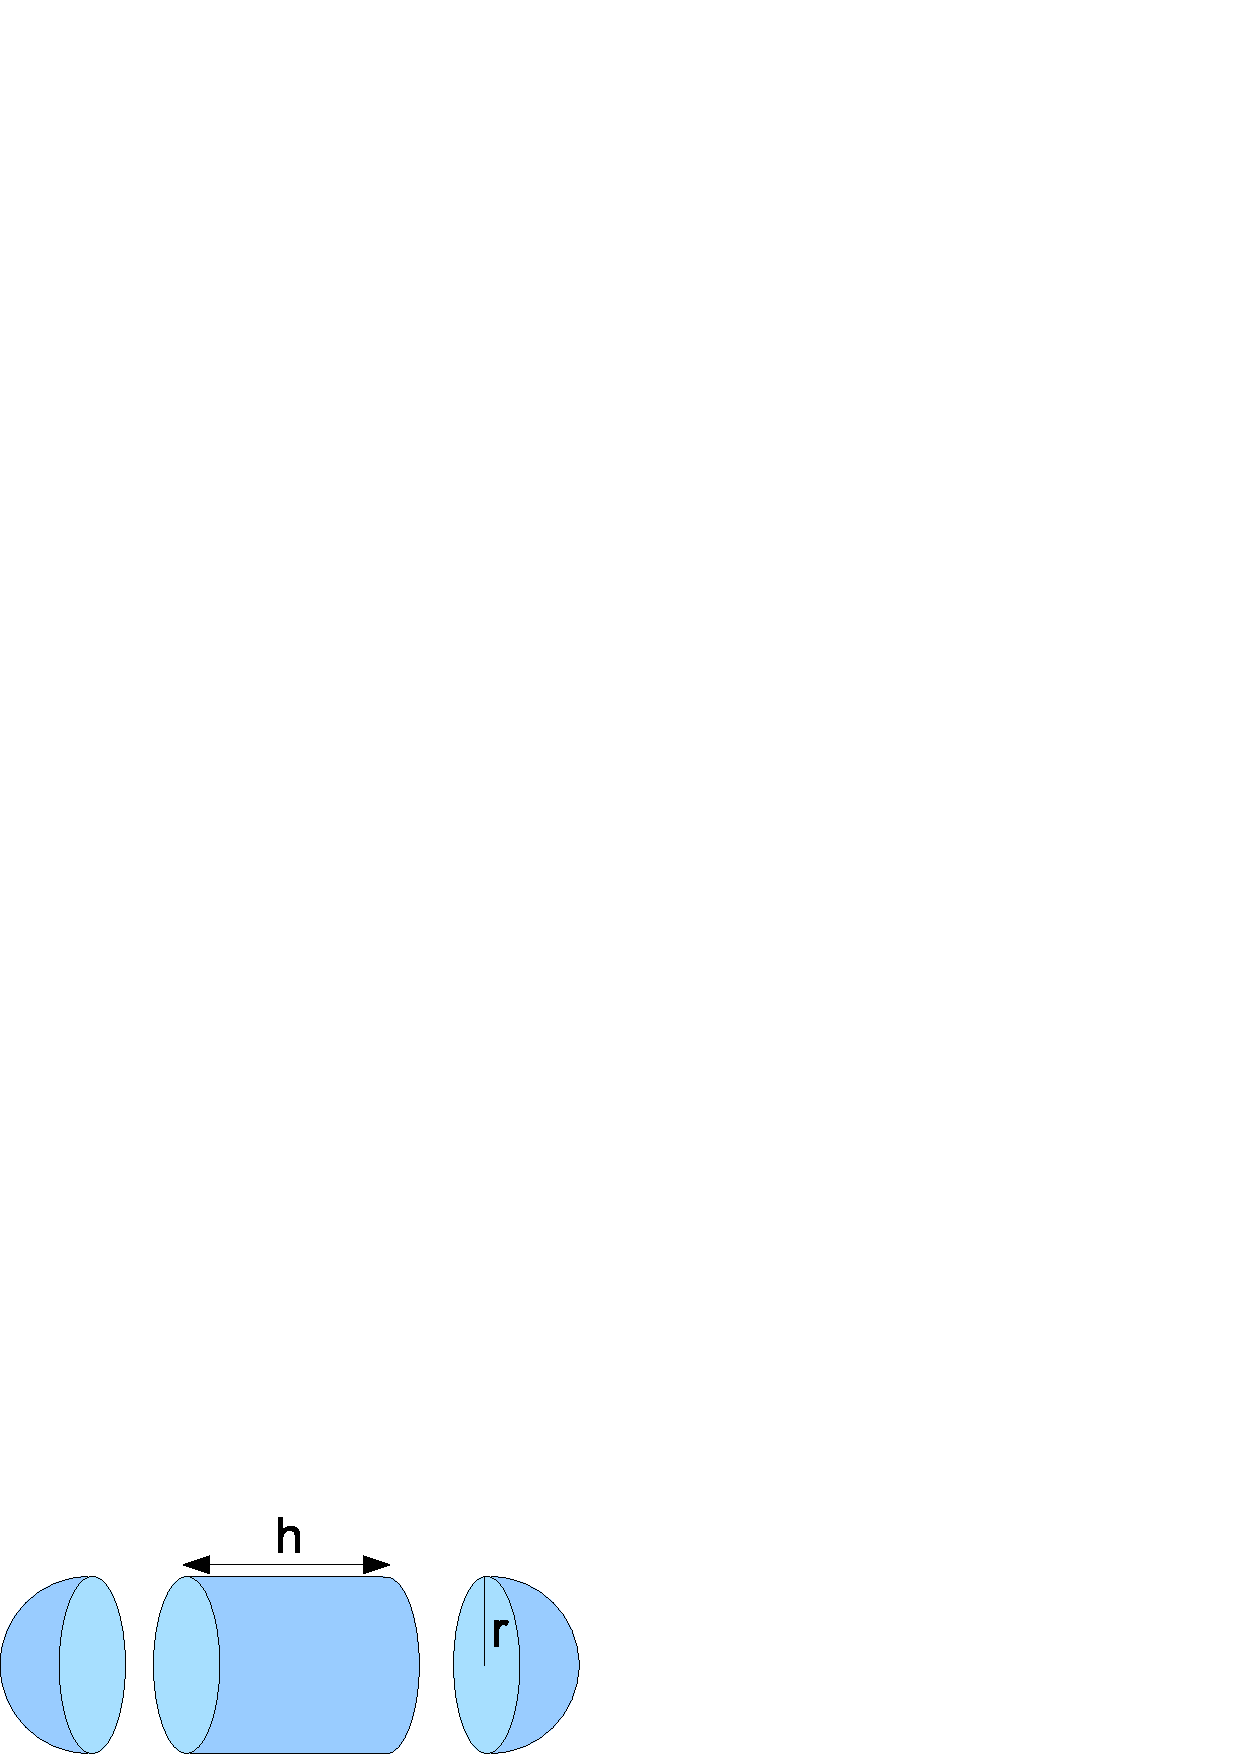
\includegraphics[scale=0.4]{img/capsula-ext-6}
\]
así que su volumen es
\[
V(r,h) = \pi r^2 h + \frac{4}{3}\pi r^3,
\]
y su superficie
\[
S(r,h) = 2\pi r h +4 \pi r^2.
\]
Como el volumen  debe ser $0.8$ cm$^3$ tenemos que
\[
V(r,h) = \pi r^2 h + \frac{4}{3}\pi r^3 = 0.8 \Leftrightarrow h = \frac{0.8-4/3\pi r^3}{\pi r^2},
\]
y sustituyendo en la fórmula de superficie tenemos
\[
S(r) = 2\pi r \frac{0.8-4/3 \pi r^3}{\pi r^2} +4 \pi r^2 = \frac{1.6-8/3\pi r^2}{r}+4\pi r^2 = \frac{1.6}{r}-\frac{8}{3}\pi r^2 +4\pi r^2 = \frac{1.6}{r^2}+\frac{4}{3}\pi r^2
\]
Como queremos que la superficie de la cápsula sea mínima, tenemos que buscar el mínimo de esta función. Para ello, calculamos primero los puntos críticos que anulan su derivada:
\[
\frac{dS}{dr} = -\frac{1.6}{r^2}+\frac{4}{3}\pi2r = 0 \Leftrightarrow \frac{1.6}{r^2} = \frac{8}{3}\pi r \Leftrightarrow \frac{8}{3}\pi r^3 = 1.6 \Leftrightarrow r^3 = \frac{1.6}{8/3 \pi} = 0.1910 \Leftrightarrow r = \sqrt[3]{0.1910} = 0.5759
\]
y por tanto la altura será
\[
h = \frac{0.8-4/3\pi r^3}{\pi r^2} = \frac{0.8-4/3\pi 0.5759^3}{\pi 0.5759^2} = 0.
\]
Esto quiere decir, que realmente no habría cilindro, y por tanto para que la supercie sea mínima la cápsula debería tener forma de esfera.

Sólo falta comprobar que el punto anterior es realmente un punto de mínimo. Para ello podemos utilizar la segunda derivada
\[
\frac{d^2S}{dr^2} = \frac{d}{dr}\left(-\frac{1.6}{r^2}+\frac{8}{3}\pi r\right) = \frac{1.6\cdot 2r}{r^4}+\frac{8}{3}\pi = \frac{3.2}{r^3}+\frac{8}{3}\pi.
\]
y sustituyendo en el punto anterior tenemos
\[
\frac{d^2S}{dr^2}(0.5759) =  \frac{3.2}{0.5759^3}+\frac{8}{3}\pi = 25.13 >0,
\]
que al tener signo positivo indica que efectivamente se trata de un mínimo.
}

\newproblem{ext-7}{gen}{*}
%ENUNCIADO
{Consider a function $f(x)$ with derivative given by
\[
f'(x) = \frac{(2-x) e^{-\frac{x^2}{2}+2x-2}}{\sqrt{2\pi}}
\]
\begin{enumerate}
\item Determine the regions on which $f$ is increasing, and those where $f$ is decreasing.
\item Find the extrema points of $f$.
\item Determine the points on which $f$ is concave up, and those on which it is concave down.
\item Find the values of $x$ corresponding to the inflection points of the graph of $f$.
\end{enumerate}
}
%SOLUCIÓN
{\begin{enumerate}
\item Increasing at $x<2$ and decreasing at $x>2$.
\item Relative maximum at $x=2$.
\item Concave down at$(-\infty,1)$ and $(3,\infty)$, and concave down at $(1,3)$.
\item Inflection points at $x=1$ and $x=3$.
\end{enumerate}
}
%RESOLUCIÓN
{
}


\newproblem{ext-8}{qui}{}
%ENUNCIADO
{The speed $v$ at which certain chemical reaction $A+B\rightarrow AB$ takes place is a function of the concentraion $x$ of the substance $AB$.
This speed it is given by the following equation:
\[
v(x) = 4(3-x)(5-x).
\]
Determine the value of $x$ that maximizes the speed of the process.
}
%SOLUCIÓN
{None.
}
%RESOLUCIÓN
{
}


\newproblem{ext-9}{amb}{}
%ENUNCIADO
{The wheat yield $C$ of a field depends on the level of nitrogen on the ground $n$, and it is given by the following relation:
\[
C(n) = \frac{n}{1+n^2},\quad n\geq 0.
\]
Find the level of nitrogen that will produce the biggest yield.
}
%SOLUCIÓN
{$n=1$.
}
%RESOLUCIÓN
{
}


\newproblem{ext-10}{amb}{}
%ENUNCIADO
{Existen organismos que se reproducen una sóla vez en su vida como por ejemplo los salmones.
En este tipo de especies, la velocidad de incremento per cápita $v$, que mide la capacidad reproductiva, depende de la edad $x$ según la ecuación
\[
v(x) = \frac{\log(p(x)h(x))}{x},
\]
donde $p(x)$ es la probabilidad de sobrevivir hasta la edad $x$ y $h(x)$ es el número de nacimientos de hembras a la edad $x$.
Calcular la edad óptima de reproducción, es decir, el valor que maximice $v$, para $p(x)=e^{-0.1x}$ y $h(x)=4x^{0.9}$.}
%SOLUCIÓN
{$x=0.58$ años.
}
%RESOLUCIÓN
{
}


\newproblem{ext-12}{amb}{}
%ENUNCIADO
{The response $S$ of an organism to a drug depends on the dose $x$ by the relation
\[
S(x) = x(C-x),
\]
where $C$ is the maximum amount of the drug that can be given to a person.
Find the dose $x$ for which the response is maximum.
}
%SOLUCIÓN
{$x=C/2$.
}
%RESOLUCIÓN
{
}

% Author: Alfredo Sánchez Alberca (asalber@ceu.es)

\newproblem*{tay-1}{gen}{}
%STATEMENT
{Consider the function $f(x)=\sqrt{x+1}$.
\begin{enumerate}
\item  Compute the Taylor polynomial of $f$, of degree $4$, centered at $x=0$.
\item Obtain two approximate values of $\sqrt{1.02}$ by means of degrees 2 and 4 Taylor polynomials.
\end{enumerate}
}


\newproblem{tay-2}{gen}{}
%STATEMENT
{Consider the sine function $f(x) = \sin x$.
\begin{enumerate}
\item Compute the third degree Taylor polynomial centered at the point $x=\pi/6$.
Use this polynomial to approximate $\sin (1/2)$. %Provide an upper bound for the error in your approximation.
\item Give an approximate value of $\sin (1/2)$ using a fifth degree Taylor polynomial centered at the point $x=0$. %Give an upper bound for the error in your approximation.
\end{enumerate}
}
%SOLUTION
{
\begin{enumerate}
\item $P^3_{f,\pi/6}(x) = \frac{1}{2}+\frac{\sqrt{3}}{2}(x-\pi/6)-\frac{1}{4}(x-\pi/6)^2-\frac{\sqrt{3}}{12}(x-\pi/6)^3$.\\
$\sen 1/2 \approx P^3_{f,\pi/6}(1/2) = 0.4794255322$.\\
%$|R^3_{f,\pi/6}(1/2)|\leq 6.46\cdot 10^{-9}$.
\item $P^5_{f,0}(x) = x -\frac{1}{6} x^3 + \frac{1}{120}x^5$.\\
$\sin 1/2 \approx P^5_{f,0}(1/2) = 0.4794270833$.\\
%$|R^5_{f,0}(1/2)|\leq 2.170\cdot 10^{-5}$.
\end{enumerate}
}
%RESOLUTION
{
}


\newproblem{tay-3}{gen}{}
%STATEMENT
{Compute the second degree Taylor polynomial of the function $f(x)=\sqrt[3]{x}$ in a neighborhood of the point $x=1$.
}
%SOLUTION
{$P^2_{f,1}(x) = 1+\frac{1}{3}(x-1)-\frac{2}{18}(x-1)^2$.
}
%RESOLUTION
{
}


\newproblem{tay-4}{gen}{}
%STATEMENT
{Compute the third degree Maclaurin polynomial for the function $f(x)=\arcsin x$.
}
%SOLUTION
{$P^3_{f,0}(x) = x+\frac{1}{6}x^3$.
}
%RESOLUTION
{
}


\newproblem*{tay-5}{gen}{}
%STATEMENT
{Compute $\cos 1$ with an error less than $10^{-7}$ using Taylor polynomials.
}


\newproblem{tay-6}{gen}{*}
%STATEMENT
{Dadas las funciones
$f(x)=e^x$ y $g(x)=\cos x$, se pide:
\begin{enumerate}
   \item  Calcular los polinomios de Maclaurin de segundo grado para $f$
   y $g$.

   \item  Utilizar los polinomios anteriores para calcular
   \[ \lim_{x\rightarrow 0}\frac{e^x-\cos x}{x}.\]
\end{enumerate}
}
%SOLUTION
{\begin{enumerate}
\item $P^2_{f,0}(x) = 1+x+\frac{1}{2}x^2$ y $P^2_{g,0}(x) = 1-\frac{1}{2}x^2$.
\item $\lim_{x\rightarrow 0}\frac{e^x-\cos x}{x} = \lim_{x\rightarrow 0}\frac{x+x^2}{x} = 1$.
\end{enumerate}
}
%RESOLUTION
{
}


\newproblem{tay-7}{far}{*}
%STATEMENT
{The function $C(t)$ measures the concentration (in mg/dl) of a drug in the bloodstream as function of time (in hours):
\[
C(t) = \frac{1}{{1 + e^{-2t}}}
\]
\begin{enumerate}
\item Compute the third degree Maclaurin polynomial for the function.

\item Use the previous polynomial to compute approximately the concentration of drug in the bloodstream after 15 minutes.
\end{enumerate}
}
%SOLUTION
{
\begin{enumerate}
\item $P_{C,0}^3(t)=\frac{1}{2}+\frac{1}{2}t+0\frac{t^2}{2!}-1\frac{t^3}{3!}=\frac{1}{2}+\frac{1}{2}t-\frac{1}{6}t^3$.
\item $P_{C,0}^3(0.25)= 0.6223958333 \mbox{ mg/dl}$.
\end{enumerate}
}
%RESOLUTION
{\begin{enumerate}
\item
La fórmula del polinomio de Maclaurin de orden 3 para la función $C(t)$ es:
\begin{equation}
\label{e:Maclaurin}
P_{C,0}^3(t)=C(0)+\frac{dC}{dt}(0)t+\frac{d^2C}{dt^2}(0)\frac{t^2}{2!}+\frac{d^3C}{dt^3}(0)\frac{t^3}{3!}
\end{equation}
Necesitamos calcular las tres primeras derivadas:
\begin{align*}
\frac{dC}{dt} &= \frac{2e^{-2t}}{(1+e^{-2t})^2},\\
\frac{d^2C}{dt^2} &=
\frac{\frac{d}{dt}(2e^{-2t})(1+e^{-2t})^2-2e^{-2t}\frac{d}{dt}(1+e^{-2t})^2}{(1+e^{-2t})^4} =\\
&= \frac{-4e^{-2t}(1+e^{-2t})^2- 2e^{-2t}2(1+e^{-2t})(-2e^{-2t})}{(1+e^{-2t})^4}
= \frac{-4e^{-2t}+4e^{-4t}}{(1+e^{-2t})^3},\\
\frac{d^3C}{dt^3}
&=
\frac{\frac{d}{dt}(-4e^{-2t}1+4e^{-4t})(1+e^{-2t})^3-(-4e^{-2t}+4e^{-4t})\frac{d}{dt}(1+e^{-2t})^3}{(1+e^{-2t})^6}=\\
&=
\frac{(8e^{-2t}-16e^{-4t})(1+e^{-2t})^3-(-4e^{-2t}+4e^{-4t})3(1+e^{-2t})^2(-2e^{-2t})}{(1+e^{-2t})^6}=\\
&=
\frac{(8e^{-2t}-16e^{-4t})(1+e^{-2t})-(-4e^{-2t}+4e^{-4t})(-6e^{-2t})}{(1+e^{-2t})^4}=\\
&=
\frac{(8e^{-2t}-8e^{-4t}-16e^{-6t})-(24e^{-4t}-24e^{-6t})}{(1+e^{-2t})^4}=\\
&=
\frac{8e^{-2t}-32e^{-4t}+8e^{-6t}}{(1+e^{-2t})^4}.
\end{align*}
Sustituyendo para $t=0$ tenemos:
\begin{align*}
C(0)&= \frac{1}{1+e^{-2\cdot 0}}=\frac{1}{2},\\
\frac{dC}{dt}(0) &= \frac{2e^{-2\cdot 0}}{(1+e^{-2\cdot 0})^2} = \frac{2}{2^2}=\frac{1}{2},\\
\frac{d^2C}{dt^2}(0) &= \frac{-4e^{-2\cdot 0}+4e^{-4\cdot 0}}{(1+e^{-2\cdot
0})^3} = \frac{-4+4}{2^3}= 0,\\
\frac{d^3C}{dt^3}(0)&=\frac{(8e^{-2\cdot 0}-32e^{-4\cdot 0}+8e^{-6\cdot 0})}{(1+e^{-2\cdot 0})^4}=\frac{8-32+8}{16}=-1.
\end{align*}

Y por último, sustituyendo en la ecuación \ref{e:Maclaurin} llegamos al polinomio
\[
P_{C,0}^3(t)=\frac{1}{2}+\frac{1}{2}t+0\frac{t^2}{2!}-1\frac{t^3}{3!}=\frac{1}{2}+\frac{1}{2}t-\frac{1}{6}t^3.
\]

\item La concentración del fármaco transcurridos 15 minutos ($0.25$ horas) es aproximadamente
\[
C(0.25)\approx P_{C,0}^3(0.25)= \frac{1}{2}+\frac{1}{2}0.25-\frac{1}{6}0.25^3= 0.6223958333 \mbox{ mg/dl}.
\]
\end{enumerate}
}


\newproblem{tay-8}{gen}{*}
%STATEMENT
{Obtener el desarrollo en serie de Taylor hasta orden tres en el punto $1$ de la función
\[f(x) = \ln\sqrt{\dfrac{x^2+1}{2}}.\]
Utilizar el polinomio obtenido calcular una aproximación de $\ln\sqrt{1.22}$ y acotar el error cometido.
}
%SOLUTION
{$P^3_{f,1}(x) = \frac{1}{2}(x-1)-\frac{1}{12}(x-1)^3$.\\
$\ln\sqrt{1.22} \approx P^3_{f,1}(1.2) = 0.0993333$.\\
$|R^3_{f,1}(1.2)|\leq 1.25\cdot 10^{-4}$.

}
%RESOLUTION
{
}


\newproblem{tay-9}{gen}{*}
%STATEMENT
{Dada la función $f(x)=\arctg(x/2)$ se pide:
\begin{enumerate}
\item Calcular el polinomio de Maclaurin de orden 3.
\item Utilizar el polinomio anterior para aproximar $\arctg 0.05$.
\item Dar una cota del error cometido.
\end{enumerate}
}
%SOLUTION
{\begin{enumerate}
\item $P^3_{f,0}(x) =  \frac{1}{2}x-\frac{1}{24}x^3$.
\item $\arctan 0.05 \approx P^3_{f,0}(0.1) = 0.0499583333$.
\item $|R^3_{f,0}(0.1)|\leq 3.08\cdot 10^{-7}$.
\end{enumerate}
}
%RESOLUTION
{
}


\newproblem{tay-10}{gen}{*}
%STATEMENT
{Dada la función $f(x)=\dfrac{1}{1-x}$ con $x\neq 1$, se pide:
\begin{enumerate}
\item Calcular el polinomio de Maclaurin de $f$ de grado 4.
\item Calcular el polinomio de Maclaurin de $f$ de grado $n$.
\item Calcular el resto de Lagrange para el polinomio de grado $n$ en el punto $x=0.03$.
\item ¿Hasta qué grado tendríamos que llegar para conseguir una aproximación de $f(0.03)$ con un error menor de $10^{-10}$?
\end{enumerate}
}
%SOLUTION
{\begin{enumerate}
\item $P^4_{f,0}(x) = 1 + x + x^2 + x^3 + x^4$.
\item $P^n_{f,0}(x) = 1 + x + x^2 + \cdots + x^n$.
\item $R^n_{f,0}(0.03) = \frac{0.03^{n+1}}{(1-t)^{n+2}} \ t\in(0,0.03)$.
\item $|R^n_{f,0}(0.03)| \leq \frac{0.03^{n+1}}{(0.97)^{n+2}}\leq 10^{-10}$ para $n\geq 6$.
\end{enumerate}
}
%RESOLUTION
{
}


\newproblem{tay-11}{gen}{*}
%STATEMENT
{Dada la función $f(x)=\tg(x/2)$, se pide:
\begin{enumerate}
\item Aproximar $\tg(0.1)$ mediante un polinomio de Taylor de grado 3 para la función $f$.
\item Dar una cota del error cometido.
\end{enumerate}
}
%SOLUTION
{
\begin{enumerate}
\item $T_3 (f,0)(0.2) = 0.1003333$.
\item ${\rm Error} \le 0.00033$.
\end{enumerate}
}
%RESOLUTION
{\begin{enumerate}
\item Sabemos que el desarrollo de Taylor de grado 3 de una función
$f$,  centrado en $a$ y en función de $x$ viene dado por:
\[
T_3 (f,a)(x) = f(a) + f'(a)(x - a) + \frac{{f''(a)}}{2}(x - a)^2  +
\frac{{f'''(a)}}{6}(x - a)^3
\]
y que el valor de la función en un cierto $x_0$, próximo a $a$,
puede calcularse de forma aproximada mediante:
\[
f(x_0 ) \approx T_3 (f,a)(x_0 )
\]
En nuestro caso, la función $f(x)= \tg x/2$ y debemos aproximar el
valor de $\tg 0.1$. Por lo tanto:
\[
\tg 0.1 = \tg \frac{{x_0 }}{2} \Leftrightarrow x_0  = 0.2
\]
Y como valor de $a$ (punto en el que centramos el polinomio de
Taylor) podemos tomar 0, ya que está lo suficientemente próximo a
$0.2$ como para que la aproximación sea buena, además de simplificar
notablemente los cálculos. Es decir, vamos a calcular el polinomio
de Maclaurin.

Entre las múltiples expresiones para la derivada de la tangente
(como cociente de senos y cosenos, con la secante y también con la
propia tangente), posiblemente la más cómoda para hacer derivadas de
orden superior es:
\[
f(x) = \tg (u(x)) \Rightarrow f'(x) = \left( {1 + \tg ^2 (u(x))}
\right)u'(x)
\]
Aplicado a nuestra función:
\[
f(x) = \tg \frac{x}{2}
\]
\[
f'(x) = \left( {1 + \tg ^2 \frac{x}{2}} \right)\frac{1}{2} =
\frac{1}{2} + \frac{1}{2}\tg ^2 \frac{x}{2}
\]

Procediendo de forma similar con las derivadas de segundo y tercer
orden, obtenemos:
\[
f''(x) = \frac{1}{2}\tg \frac{x}{2} + \frac{1}{2}\tg ^3
\frac{x}{2}
\]
\[
f'''(x) = \frac{1}{4} + \tg ^2 \frac{x}{2} + \frac{3}{4}\tg ^4
\frac{x}{2}
\]
Por lo tanto:
\[
f(0) = 0;\;f'(0) = 1/2;\;f''(0) = 0;\;f'''(0) = 1/4
\]
Con ello, el polinomio de Maclaurin buscado es:
\[
T_3 (f,0)(x) = \frac{1}{2}x + \frac{1}{{24}}x^3
\]

Y la aproximación buscada vale:
\[
\tg 0.1 \approx T_3 (f,0)(0.2) = \frac{1}{2}\;0.2 +
\frac{1}{{24}}\;0.2^3  = 0.1003333
\]
Para comprobar que la aproximación obtenida es correcta, mediante
calculadora, utilizando como unidad angular el radián, obtenemos:
$\tg 0.1=0.1003346$


\item Sabemos que el error cometido con la anterior aproximación es
igual al valor absoluto del resto, y que este último viene dado por
la fórmula:
\[
R_n (f,a)(x) = \frac{{f^{(n + 1} (t)}}{{(n + 1)!}}(x - a)^{n + 1}
\]
donde $t$ pertenece al intervalo $(a,x)$ si $x>a$, o a $(x,a)$ si
$a>x$.
En nuestro caso:
\[
R_3 (f,0)(0.2) = \frac{{f^{(4} (t)}}{{4!}}(0.2)^{4}
\]
Si tenemos en cuenta que la derivada cuarta vale:
\[
f^{(4} (x) = \tg \frac{x}{2} + \frac{5}{2}\tg ^3 \frac{x}{2} +
\frac{3}{4}\tg ^5 \frac{x}{2} \Rightarrow f^{(4} (t) = \tg
\frac{t}{2} + \frac{5}{2}\tg ^3 \frac{t}{2} + \frac{3}{4}\tg ^5
\frac{t}{2}
\]
obtenemos:
\[
R_3 (f,0)(0.2) = \frac{{\tg \frac{t}{2} + \frac{5}{2}\tg ^3
\frac{t}{2} + \frac{3}{4}\tg ^5 \frac{t}{2}}}{{24}}\,(0.2)^4 ;\quad
t \in (0,\;0.2)
\]
Por lo tanto el error cometido vale:
\[
\left| {\frac{{\tg \frac{t}{2} + \frac{5}{2}\tg ^3 \frac{t}{2} +
\frac{3}{4}\tg ^5 \frac{t}{2}}}{{4!}}\,(0.2)^4 } \right|;\quad t
\in (0,\;0.2)
\]
Y nos piden que acotemos el error, es decir, que encontremos una
cierta cantidad tal que se demuestre que el error es menor o igual
que esa cantidad. Para ello, nos damos cuenta de que la función
tangente, e igualmente la tangente al cubo o a la quinta potencia,
son funciones crecientes en el intervalo $(0,\,0.2)$ y, por lo
tanto, el error alcanzará su máximo valor posible cuando $t$ sea un
valor muy próximo a $0.2$. No obstante obtenemos un error en cuya
expresión aparece de nuevo la tangente de $0.1$, y no tiene ningún
sentido utilizar la calculadora para calcular la tangente de $0.1$
presente en el resto, cuando precisamente es la tangente de $0.1$ lo
que pretendemos calcular mediante el polinomio de Taylor. No
obstante, podemos utilizar otras cotas menos precisas pero que
supongan cálculos fácilmente realizables sin necesidad de
calculadora, y evitando a la vez el que la tangente de $0.1$
aparezca en el error. Por ejemplo, la más sencilla se obtiene
considerando que en el intervalo $(0,\,0.2)$ $\tg(t/2)\leq 1$, e
igualmente la tangente cubo o a la quinta potencia.

Teniendo en cuenta lo anterior:
\[
{\rm Error} \le \frac{{(0.2)^4 }}{{4!}}\left| {1 + \frac{5}{2} +
\frac{3}{4}\,} \right| = 0.00033
\]
Una cota más precisa se obtiene tomando, por ejemplo, $t=\pi/3$, tal
que la tangente de $\pi/6$ sí que tiene un valor fácilmente
calculable (sin calculadora):
\[
\tg \frac{\pi }{6} = \frac{{1/2}}{{\sqrt 3 /2}} = \frac{{\sqrt 3
}}{3}
\]
Con ello, la cota para el error cometido vale:
\[
{\rm Error} \le \frac{{(0.2)^4 }}{{4!}}\left| {1\frac{{\sqrt 3 }}{3}
+ \frac{5}{2}\left( {\frac{{\sqrt 3 }}{3}} \right)^3  +
\frac{3}{4}\left( {\frac{{\sqrt 3 }}{3}} \right)^5 \,} \right| =
0.000077
\]
\end{enumerate}
}


\newproblem{tay-12}{gen}{*}
%STATEMENT
{Dada  la función $f(x) = 2\sqrt[3]{{1 + x}}$, se pide:
\begin{enumerate}
\item Hallar el polinomio de Maclaurin de tercer grado de la función.
\item Utilizar el polinomio obtenido en el apartado anterior para calcular un valor aproximado de $\sqrt[3]{9}$.
\item Dar una cota del error cometido.
\end{enumerate}
}
%SOLUTION
{\begin{enumerate}
\item $P(3,f,0)(x)=2+\frac{2}{3}x-\frac{2}{9}x^2+\frac{10}{81}x^3$.
\item $P(3,f,0)(0.125)= 2.080102258$.
\item $|R_{3,f,0}(0.125)| \leq 2.00938\cdot 10^{-5}$.
\end{enumerate}
}
%RESOLUTION
{\begin{enumerate}
\item   La fórmula del polinomio de Maclaurin de orden $3$ para la
    función $f$ es
\begin{equation}
    P_{3,f,0} (x)= f(0)+
    f'(0)x+\frac{f''(0)}{2!}x^2+\frac{f'''(0)}{3!}x^3,
    \label{Maclaurin}
\end{equation}
de modo que tenemos que calcular hasta la tercera derivada de $f$ en el 0.
\[ \renewcommand{\arraystretch}{2}
    \begin{array}{lll}
        f(x)=2\sqrt[3]{{1 + x}}=2(1+x)^{1/3}, & \quad \quad & f(0)=2(1+0)^{1/3}=2,  \\
        f'(x)=2\dfrac{1}{3}(1+x)^{-2/3}=\dfrac{2}{3}(1+x)^{-2/3}, &  & f'(0)=\dfrac{2}{3}(1+0)^{-2/3}=\dfrac{2}{3},\\
        f''(x)=\dfrac{2}{3}\dfrac{-2}{3}(1+x)^{-5/3}=\dfrac{-4}{9}(1+x)^{-5/3}, &  & f''(0)=\dfrac{-4}{9}(1+0)^{-5/3}=\dfrac{-4}{9},\\
        f'''(x)=\dfrac{-4}{9}\dfrac{-5}{3}(1+x)^{-8/3}=\dfrac{20}{27}(1+x)^{-8/3}, &  & f'''(0)=\dfrac{20}{27}(1+0)^{-8/3}=\dfrac{20}{27},
     \end{array}
\]
Sustituyendo estos valores en la ecuación \ref{Maclaurin},
obtenemos el polinomio que nos piden
\[
P(3,f,0)(x)= 2+\frac{2}{3}x+\frac{-4/9}{2}x^2+\frac{20/27}{6}x^3=
2+\frac{2}{3}x-\frac{2}{9}x^2+\frac{10}{81}x^3.
\]

\item Primero averiguamos en qué punto la función vale $\sqrt[3]{9}$.
\[
f(x)=2\sqrt[3]{1+x}=\sqrt[3]{9} \Leftrightarrow (2\sqrt[3]{1+x})^3=(\sqrt[3]{9})^3 \Leftrightarrow
2^3(1+x)=9 \Leftrightarrow 8+8x=9 \Leftrightarrow x=\frac{1}{8}=0.125.
\]
Calculando el polinomio anterior en este punto tenemos
\[
\sqrt[3]{9}\approx P(3,f,0)(0.125)= 2+\frac{2}{3}0.125-\frac{2}{9}0.125^2+\frac{10}{81}0.125^3=2.080102258.
\]

\item El error cometido en la aproximación anterior nos lo da el resto de Taylor, que en la forma
Lagrange es
\[
R_{3,f,0}(x)=\frac{f^{iv}(t)}{4!}x^4=\frac{\frac{160}{81} (1+t)^{-11/3}}{24}x^4 = \frac{20}{243}\frac{1}{(1+t)^{11/3}} x^4 \quad t\in(0,x),
\]
En el punto $x=0.125$ donde hemos calculado la aproximación, vale
\[
R_{3,f,0}(0.125)=\frac{20}{243}\frac{1}{(1+t)^{11/3}} 0.125^4= 2.00938\cdot 10^{-5}\frac{1}{(1+t)^{11/3}} \quad t\in(0\,,\,0.125).
\]
Para acotar el resto, basta con calcular el máximo de esta función en el
intervalo $(0\,,\,0.125)$. Puesto que la función $1/(1+t)^{11/3}$ es decreciente en dicho intervalo,
el máximo se alcanza en el extremo inferior del intervalo, es decir,
$t=0$. Así pues, tenemos la siguiente cota
\[
|R_{3,f,0}(0.125)|=|2.00938\cdot 10^{-5}\frac{1}{(1+t)^{11/3}}|\leq
|2.00938\cdot 10^{-5}\frac{1}{(1+0)^{11/3}}|=2.00938\cdot 10^{-5}.
\]
\end{enumerate}
}


\newproblem{tay-13}{gen}{*}
%STATEMENT
{Dada la función: $f(x) = \dfrac{2} {{\sqrt {3x+ 1} }}$
\begin{enumerate}
\item Obtener el polinomio de Maclaurin de tercer grado.
\item Calcular el valor aproximado de $\dfrac{2}{1,3}$ empleando el polinomio anterior.
\end{enumerate}
}
%SOLUTION
{\begin{enumerate}
\item $P(3,f,0)(x)= 2-3x+\frac{27}{4}x^2-\frac{135}{8}x^3$.
\item $\frac{2}{1.3}\approx P(3,f,0)(0.23)=1.461756910$.
\end{enumerate}
}
%RESOLUTION
{\begin{enumerate}
\item   La fórmula del polinomio de Maclaurin de orden $3$ para la función $f$ es
\begin{equation}
P_{3,f,0} (x)= f(0)+ f'(0)x+\frac{f''(0)}{2!}x^2+\frac{f'''(0)}{3!}x^3,
\label{Maclaurin}
\end{equation}
de modo que tenemos que calcular hasta la tercera derivada de $f$ en el 0.
\[ \renewcommand{\arraystretch}{2}
    \begin{array}{ll}
        f(x)=\dfrac{2}{\sqrt{3x+1}}= 2(3x+1)^{-1/2}, & f(0)=2(3\cdot 0+1)^{-1/2}=2,  \\
        f'(x)=2\dfrac{-1}{2}(3x+1)^{-3/2}3=-3(3x+1)^{-3/2}, &  f'(0)=-3(3\cdot 0+1)^{-3/2}=-3,\\
        f''(x)=-3\dfrac{-3}{2}(3x+1)^{-5/2}3=\dfrac{27}{2}(3x+1)^{-5/2}, &  f''(0)=\dfrac{27}{2}(3\cdot 0+1)^{-5/2}=\dfrac{27}{2},\\
        f'''(x)=\dfrac{27}{2}\dfrac{-5}{2}(3x+1)^{-7/2}3=\dfrac{-405}{4}(3x+1)^{-7/2}, & f'''(0)=\dfrac{-405}{4}(3\cdot 0+1)^{-7/2}=\dfrac{-405}{4},
     \end{array}
\]
Sustituyendo estos valores en la ecuación \ref{Maclaurin}, obtenemos el polinomio que nos piden
\[
P(3,f,0)(x)= 2-3x+\frac{27/4}{2!}x^2-\frac{405/24}{3!}x^3=
2-3x+\frac{27}{4}x^2-\frac{135}{8}x^3.
\]

\item Primero averiguamos en qué punto la función vale $2/1.3$.
\[
f(x)=\frac{2}{\sqrt{3x+1}}=\frac{2}{1.3} \Leftrightarrow \sqrt{3x+1}=1.3 \Leftrightarrow
3x+1=1.3^2=1.69 \Leftrightarrow x=\frac{0.69}{3}=0.23.
\]
Calculando el polinomio anterior en este punto tenemos
\[
\frac{2}{1.3}\approx P(3,f,0)(0.23)= 2-3\cdot 0.23+\frac{27}{4}0.23^2-\frac{135}{8}0.23^3=1.461756910.
\]
\end{enumerate}
}


\newproblem*{tay-14}{gen}{*}
%STATEMENT
{Sea la función
\[
f(x) = 2\sqrt[4]{{1 + x}}
\]
\begin{enumerate}
\item Calcular su desarrollo de Maclaurin de orden 3.
\item Utilizar el desarrollo anterior para calcular de forma aproximada: $\sqrt[4]{{16,16}}$.
\item Acotar el error cometido con la aproximación anterior.
\end{enumerate}
}


\newproblem*{tay-15}{gen}{*}
%STATEMENT
{
Sea la función $f(x)=x^{x}.$
\begin{enumerate}
\item  Calcular su polinomio de Taylor de segundo orden, centrado en $x=1$.
\item  Aproximar con dicho polinomio el valor de: $1.1^{1.1}$.
\end{enumerate}
}


\newproblem*{tay-16}{gen}{*}
%STATEMENT
{Para la función:
\[
f(x)=\sqrt[3]{1+2x}
\]
Calcular:
\begin{enumerate}
\item  Su polinomio de Taylor de tercer orden centrado en 0.
\item  El valor aproximado de $\sqrt[3]{1.2}$ mediante el polinomio de Taylor calculado anteriormente.
\item  Acotar el error cometido mediante dicha aproximación.
\end{enumerate}
}


\newproblem*{tay-17}{gen}{*}
%STATEMENT
{Teniendo en cuenta que $\sen (2x)=2\sen x \cos x$ y los desarrollos de McLarin de las funciones $\sen x$ y $\cos x$, ¿cuál será el desarrollo de Maclaurin de orden 3 para la función $\sen (2x)$?

Calcular directamente el desarrollo de Maclaurin de orden 3 de la función $\sen (2x)$ para comprobar el resultado obtenido en el apartado anterior.
}


\newproblem*{tay-18}{gen}{*}
%STATEMENT
{En los libros de Cálculo se afirma que la función binómica, $(1+x)^p$, puede desarrollarse desarrollada mediante una serie de sumandos de la forma:
\[
\left( {1 + x} \right)^p  = 1 + px + \frac{{p(p - 1)}} {{2!}}x^2 + \frac{{p(p - 1)(p - 2)}} {{3!}}x^3  +  \cdots  + \frac{{p(p - 1) \cdots (p - k + 1)}} {{k!}}x^k
\]
para todo $x$ si $p$ es un entero no negativo.
\begin{enumerate}
\item Demostrar dicha fórmula hasta el término en $x^4$ mediante el desarrollo de Maclaurin de orden 4.
\item Utilizar el resultado anterior para calcular de forma aproximada el valor de: $0.9^6$.
\end{enumerate}
}


\newproblem{tay-19}{gen}{*}
%STATEMENT
{La concentración de un fármaco en sangre, en mg/dl, en función del tiempo, en horas, viene dada por la expresión:
\[
C(t) = \ln \left( {\frac{{t^2  + 2t + 1}}{{2t + 1}}} \right)
\]
Se pide:
\begin{enumerate}
\item Calcular el polinomio de Maclaurin de orden 3 de $C$.
\item Utilizar el polinomio anterior para dar el valor aproximado de la concentración al cabo de 15 minutos.
\item Calcular el polinomio de Taylor, centrado en 0, de orden 2 para la función:
\[
f(t) = 2\ln (t + 1) - \ln (2t + 1)
\]
\end{enumerate}
}
%SOLUTION
{\begin{enumerate}
\item $P_{C,0}^3(t) = t^2-2t^3$.
\item $P_{C,0}^3(0.25) = 0.03125$.
\item $P_{f,0}^2(t) = t^2$.
\end{enumerate}}
%RESOLUTION
{\begin{enumerate}
\item La ecuación del polinomio de Maclaurin de orden 3 de $C$ es
\begin{equation}
P_{C,0}^3(t) = C(0)+ C'(0)t + \frac{C''(0)}{2}t^2 + \frac{C'''(0)}{3!}t^3.
\end{equation}
Necesitamos calcular las 3 primeras derivadas, pero antes conviene simplificar la función
\begin{align*}
C(t)&= \ln\left(\frac{t^2+2t+1}{2t+2}\right)= \ln(t^2+2t+1)-\ln(2t+1) =\\
&= \ln((t+1)^2) -\ln(2t+1) = 2\ln(t+1)-\ln(2t+1),\\
C'(t)&= \frac{2}{t+1}-\frac{2}{2t+1},\\
C''(t)&= \frac{-2}{(t+1)^2}+\frac{4}{(2t+1)^2},\\
C'''(t)&= \frac{4}{(t+1)^3}-\frac{16}{(2t+1)^3}
\end{align*}
Las derivadas en 0 valen
\begin{align*}
C(0)&=  2\ln(1)-\ln(1) = 0,\\
C'(0)&= \frac{2}{1}-\frac{2}{1}= 0,\\
C''(0)&= \frac{-2}{1^2}+\frac{4}{1^2} = 2,\\
C'''(t)&= \frac{4}{1^3}-\frac{16}{1^3} = -12.
\end{align*}
Y sustituyendo en la ecuación anterior llegamos al polinomio
\[
P_{C,0}^3(t) = \frac{2}{2}t^2 - \frac{12}{3!}t^3 = t^2-2t^3.
\]

\item El valor de la función a los 15 minutos es $C(0.25)$ ya que las unidades del tiempo se consideran en horas. El valor aproximado de que da el polinomio en ese instante es
\[
P_{C,0}^3(0.25) = 0.25^2-2\cdot 0.25^3 = 0.03125.
\]

\item Según hemos podido comprobar al simplificar $C(t)$ resulta que $C(t)$ y $f(t)$ son la misma función, así que el polinomio de Maclaurin de orden 2 es el mismo que el calculado en el primer apartado pero considerando sólo hasta el término de grado 2, es decir,
\[
P_{f,0}^2(t) = t^2.
\]
\end{enumerate}
}


\newproblem{tay-20}{gen}{}
%STATEMENT
{Dada la función $\dfrac{\sen x+\cos x}{2}$:
\begin{enumerate}
\item  Utilizar el polinomio de Maclaurin de grado 3 para aproximar $\frac{\sen 1+\cos 1}{2}$.
\item  Utilizar el polinomio de Taylor de grado 2 en el punto $x_0 = \pi/2$ para aproximar $\frac{\sen 1+\cos 1}{2}$.
\item  Dar la cota de error cometida en ambas aproximaciones y decir cual es mejor.
\end{enumerate}
}
%SOLUTION
{\begin{enumerate}
\item $P_0^3(x)=\frac{1}{2}+\frac{1}{2}x-\frac{1}{4}x^2-\frac{1}{12}x^3$ y $P_0^3(1)=\frac{2}{3}$.
\item $P_{\pi/2}^2(x)=\frac{1}{2}-\frac{1}{2}(x-\pi/2)-\frac{1}{4}(x-\pi/2)^2$ y  $P_{\pi/2}^2(1)= 0.70395$.
\item $|R_0^3(1)|\leq 0.04166$ y $|R_{\pi/2}^2(1)|\leq 0.03099$.
\end{enumerate}
}
%RESOLUTION
{\begin{enumerate}
\item  El polinomio de Maclaurin de grado 3 para $f(x)$ viene dado por la fórmula siguiente:
\[
P_0^3(x)=f(0)+f^{\prime }(0)x+\frac{f^{\prime \prime }(0)}{2!}x^2+\frac{f^{\prime \prime \prime }(0)}{3!}x^3.
\]

Calculamos las tres primeras derivadas de $f(x)$:
\begin{align*}
f^{\prime }(x) &= \frac{\cos x-\sen x}{2}, \\
f^{\prime \prime }(x) &= \frac{-\ sen x-\cos x}{2}, \\
f^{\prime \prime \prime }(x) &= \frac{-\cos x+\sen x}{2}.
\end{align*}

Particularizando en $x=0$ tenemos:
\begin{align*}
f(0) &= \frac{\sen 0+\cos 0}2=\frac{1}{2}, \\
f^{\prime }(0) &= \frac{\cos 0-\sen 0}{2}=\frac{1}{2}, \\
f^{\prime \prime }(0) &= \frac{-\sen 0-\cos 0}{2}=-\frac{1}{2}, \\
f^{\prime \prime \prime }(0) &= \frac{-\cos 0+\sen 0}{2}=-\frac{1}{2}.
\end{align*}

Por tanto, el polinomio de Maclaurin que nos interesa es:
\[
P_0^3(x)=\frac{1}{2}+\frac{1}{2}x-\frac{1}{4}x^2-\frac{1}{12}x^3.
\]

Para aproximar $f(1)=\frac{\sen 1+\cos 1}{2}$, tenemos que tomar $x=1$, y en ese punto, la aproximación que da el polinomio es:
\[
P_0^3(1)=\frac{1}{2}+\frac{1}{2}-\frac{1}{4}-\frac{1}{12}=\frac{2}{3}.
\]

\item  El polinomio de Taylor de grado 2 en el punto $x_0=\pi/2$ para $f(x)$ viene dado por la fórmula siguiente:
\[
P_{\pi /2}^2(x)=f(\pi /2)+f^{\prime }(\pi /2)(x-\pi /2)+\frac{f^{\prime\prime }(\pi /2)}{2!}(x-\pi /2)^2.
\]

Particularizando en $x=\pi/2$ hasta la segunda derivada tenemos:
\begin{align*}
f(\pi /2) &= \frac{\sen\pi/2+\cos \pi /2}{2} = \frac{1}{2} \\
f^{\prime }(\pi/2) &= \frac{\cos \pi /2-\sen\pi/2}{2} = -\frac{1}{2}, \\
f^{\prime \prime}(\pi/2) &= \frac{-\sen\pi/2-\cos\pi/2}{2} = -\frac{1}{2}.
\end{align*}

Por tanto, el polinomio de Taylor que nos interesa es:
\[
P_{\pi/2}^2(x)=\frac{1}{2}-\frac{1}{2}(x-\pi/2)-\frac{1}{4}(x-\pi/2)^2,
\]

y, de nuevo, tomando $x=1$, la aproximación que da este polinomio para $f(1)=\frac{\sen 1+\cos 1}2$ es:
\[
P_{\pi/2}^2(1)=\frac 12-\frac{1}{2}(1-\pi/2)-\frac{1}{4}(1-\pi/2)^2 = 0.70395.
\]

\item  El error cometido en las aproximaciones se puede calcular mediante el resto de Lagrange. Para el polinomio de Maclaurin anterior, dicho resto se puede calcular con la fórmula siguiente:
\[
R_0^3(x) = \frac{f^{iv}(c)}{4!}x^4\qquad \mbox{con }c\in (0,x).
\]

Como la cuarta derivada de $f(x)$ coincide con $f(x)$, entonces particularizando el resto en $x=1$, tenemos:
\[
R_0^3(1)=\frac{\sen c+\cos c}{2\cdot 4!}1^4 = \frac{\sen c+\cos c}{48} \qquad \text{con }c\in (0,1),
\]
y puesto que tanto el seno como el coseno no pueden tomar valores mayores que 1, tenemos que $|\sen c+\cos c|\leq 2$, y obtenemos la siguiente cota de error para la primera aproximaci\'{o}n:
\[
|R_0^3(1)|\leq |\frac{2}{48}|=0.04166.
\]

Para el polinomio de Taylor, el resto de Lagrange tiene la forma siguiente:
\[
R_{\pi/2}^2(x)=\frac{f^{\prime \prime \prime }(c)}{3!}(x-\pi/2)^3\qquad \mbox{con }c\in (x,\pi /2).
\]

Como antes, particularizando en $x=1$ tenemos:
\[
R_{\pi/2}^2(1)=\frac{-\cos c+\sen c}{2\cdot 3!}(1-\pi/2)^3 \qquad \mbox{con }c\in (1,\pi /2),
\]
y como $|\sen c+\cos c|\leq 2,$ obtenemos la siguiente cota de error para la segunda aproximación:
\[
|R_{\pi/2}^2(1)|\leq |\frac{2}{2\cdot 3!}(1-\pi/2)^3|=0.03099.
\]

Podemos concluir que la segunda aproximación es mejor que la primera.
\end{enumerate}
}


\newproblem{tay-21}{gen}{*}
%STATEMENT
{Calcular el polinomio de Maclaurin de orden 4 de la función $\cos\frac{x}{3}$, y utilizarlo para aproximar $\cos\frac{\pi}{4}$, dando una
cota del error cometido.
}
%SOLUTION
{$P_0^4(x)=1-\dfrac{1}{18}x^2+\dfrac{1}{1944}x^4$, $P_0^4\left(\dfrac{3\pi }{4}\right) = 0.7074292$ y la cota del error cometido es $\left|R_0^4\left(\dfrac{3\pi}{4}\right)\right| \leq 0.00249.$
}
%RESOLUTION
{Llamando $f(x)=\cos\dfrac{x}{3}$, el polinomio que se nos pide viene dado por la fórmula siguiente:
\[
P_0^4(x)=f(0)+f^{\prime }(0)x+\frac{f^{\prime \prime }(0)}{2!}x^2+\frac{f^{\prime \prime \prime }(0)}{3!}x^3+\frac{f^{\text{iv}}(0)}{4!}x^4.
\]
Calculamos primero hasta la derivada cuarta de $f(x)$:
\[
\begin{array}{lll}
f(x)=\cos\dfrac{x}{3} & \qquad & f(0)=1 \\
f^{\prime }(x)=-\dfrac{1}{3}\sen\dfrac{x}{3} & &  f^{\prime }(0)=0 \\
f^{\prime \prime }(x)=-\dfrac{1}{9}\cos\dfrac{x}{3} &  & f^{\prime \prime }(0)=-\dfrac{1}{9}\\
f^{\prime \prime \prime}(x)=\dfrac{1}{27}\sen\dfrac{x}{3} & &  f^{\prime \prime \prime }(0)=0 \\
f^{iv}(x)=\dfrac{1}{81}\cos\dfrac{x}{3} & & f^{iv}(0)=\dfrac{1}{81}
\end{array}
\]
Sustituyendo estas derivadas en la fórmula anterior obtenemos el polinomio que buscamos:
\[
P_0^4(x)=1-\dfrac{1}{18}x^2+\frac{1}{1944}x^4.
\]
Para aproximar ahora $\cos\frac{\pi}{4}$ utilizando este polinomio, tenemos que calcular el valor del polinomio para un $x$ tal que $f(x)=\cos\frac{\pi}{4},$ es decir, un $x$ tal que $\cos\frac{x}{3}=\cos\frac{\pi}{4},$ de lo que se deduce $x=\frac{3\pi}{4}$. La aproximación que da el polinomio en este punto es
\[
P_0^4\left(\dfrac{3\pi }{4}\right)=1-\dfrac{1}{18}\left(\dfrac{3\pi}{4}\right)^2+\frac{1}{1944}\left(\dfrac{3\pi}{4}\right)^4=0.7074292
\]
Finalmente, el error cometido en esta aproximación lo da el resto de Langrange que se obtiene con la fórmula
\[
R_0^4\left(\dfrac{3\pi}{4}\right)=\frac{f^{v}(t)}{5!}\left(\dfrac{3\pi}{4}\right)^5\quad \text{con }t\in \left(0,\frac{3\pi}{4}\right).
\]
Calculando la quinta derivada de $f(t),$
\[
f^{v}(t)=-\dfrac{1}{243}\sen\dfrac{t}{3},
\]
y sustitutyendo en la fórmula anterior, obtenemos el error cometido:
\[
R_0^4\left(\dfrac{3\pi}{4}\right)=-\dfrac{\sen(t/3)}{29160}\left(\dfrac{3\pi}{4}\right)^5\quad \text{con }t\in \left(0,\frac{3\pi}{4}\right).
\]
Este error puede acotarse fácilemente aprovechando que $\left|\sen(t/3)\right| \leq 1,$ con lo que llegamos a la cota
\[
\left|R_0^4\left(\dfrac{3\pi}{4}\right)\right| \leq \left|-\dfrac{1}{29160}\left(\dfrac{3\pi}{4}\right)^5\right| = 0.00249.
\]
}


\newproblem{tay-22}{gen}{*}
%STATEMENT
{Calcular $0.98^{3/5}$ tomando hasta el término correspondiente a $n=3$ del desarrollo de Mac Laurin de la función $(1+x)^{3/5}$.
}
%SOLUTION
{$P_{0}^{3}(x)=1+\dfrac{3}{5}x-\dfrac{3}{25}x^{2}+\dfrac{7}{125}x^{3}$ y $0.98^{3/5}\approx P_{0}^{3}(-0.02)= 0.9879515521$.
}
%RESOLUTION
{Llamando $f(x)=(1+x)^{3/5}$, el polinomio que se nos pide viene dado por la fórmula siguiente:
\[
P_{0}^{3}(x)=f(0)+f^{\prime }(0)x+\frac{f^{\prime \prime }(0)}{2!}x^{2}+\frac{f^{\prime \prime \prime }(0)}{3!}x^{3}.
\]

Calculamos primero hasta la derivada tercera de $f(x)$ en el $0$:
\[
\renewcommand{\arraystretch}{2}
\begin{array}{lll}
f(x)=(1+x) ^{3/5} & \qquad & f(0)=1 \\
f^{\prime}(x)=\dfrac{3}{5}(1+x)^{-2/5} & & f^{\prime }(0)=\dfrac{3}{5}\\
f^{\prime \prime}(x)=-\dfrac{6}{25}(1+x)^{-7/5} & & f^{\prime \prime }(0)=-\dfrac{6}{25}\\
f^{\prime \prime \prime}(x)=\dfrac{42}{125}(1+x)^{-12/5} & & f^{\prime \prime \prime }(0)=\dfrac{42}{125}
\end{array}
\]

Sustituyendo estas derivadas en la fórmula anterior obtenemos el polinomio que buscamos:
\[
P_{0}^{3}(x)=1+\dfrac{3}{5}x-\dfrac{3}{25}x^{2}+\frac{7}{125}x^{3}.
\]

Para aproximar $0.98^{3/5}$ usando este polinomio, tenemos que calcular el valor del polinomio para un $x$ tal que $f(x)=0.98^{3/5}$, es decir, un $x$ tal que $0.98^{3/5}=(1+x)^{3/5}$, de lo que se deduce que $x=-0.02$. La aproximación que da el polinomio en este punto es
\[
P_{0}^{3}(-0.02)=1+\dfrac{3}{5}(-0.02)-\dfrac{3}{25}(-0.02)^{2}+\frac{7}{125}(-0.02)^{3}=0.9879515521.
\]
}


\newproblem{tay-23}{gen}{*}
%STATEMENT
{Obtener polinomio de Maclaurin de grado 3 de las funciones $\sen x$ y $\tg x$, y utilizar los polinomios anteriores para calcular
\[
\lim_{x\rightarrow 0}\frac{\tg x-x}{x-\sen x}
\]
}
%SOLUTION
{$P_{0}^{3}(x)=0+1\cdot x+\frac{0}{2!}x^{2}+\frac{-1}{3!}x^{3}=x-\frac{x^{3}}{6}$,\\
$Q_{0}^{3}(x)=0+1\cdot x+\frac{0}{2!}x^{2}+\frac{2}{3!}x^{3}=x+\frac{x^{3}}{3}$ y \\
$\lim_{x\rightarrow 0}\frac{\tg x-x}{x-\sen x} = \lim_{x\rightarrow 0}\frac{x+\frac{x^{3}}{3}-x}{x-x+\frac{x^{3}}{6}} =2$.
}
%RESOLUTION
{La formula general para calcular el polinomio de Maclaurin de grado 3 de una función $f(x)$ es:
\[
P_{0}^{3}(x)=f(0)+f^{\prime }(0)x+\frac{f^{\prime \prime }(0)}{2!}x^{2}+\frac{f^{\prime \prime \prime }(0)}{3!}x^{3}.
\]

Consideremos, en primer lugar, la función $\sen x$, y calculemos sus tres primeras derivadas en 0:
\[
\begin{array}{lll}
f(x)=\sen x &  & f(0)=\sen 0=0, \\
f^{\prime }(x)=\cos x &  & f^{\prime }(0)=\cos 0=1, \\
f^{\prime \prime }(x)=-\sen x &  & f^{\prime \prime }(0)=-\sen0=0, \\
f^{\prime \prime \prime }(x)=-\cos x &  & f^{\prime \prime \prime }(0)=-\cos 0=-1.
\end{array}
\]
Sustituyendo en la fórmula de arriba, llegamos al primer polinomio que buscamos:
\[
P_{0}^{3}(x)=0+1\cdot x+\frac{0}{2!}x^{2}+\frac{-1}{3!}x^{3}=x-\frac{x^{3}}{6}.
\]

Consideremos ahora la función $\tg x$ y calculemos sus tres primeras derivadas en 0:
\[
\begin{array}{lll}
g(x)=\tg x &  & g(0)=\tg 0=0 \\
g^{\prime }(x)=1+\tg^{2} x &  & g^{\prime }(0)=1+\tg^{2} 0=1 \\
g^{\prime \prime }(x)= 2\tg x+2\tg ^{3}x &  & g^{\prime \prime}(0)= 2\tg 0+2\tg ^{3}0=0 \\
g^{\prime \prime \prime }(x)=2+ 8\tg ^{2}x+6\tg ^{4}x &  & g^{\prime \prime \prime }(0)= 2+ 8\tg ^{2}0+6\tg ^{4}0=2
\end{array}
\]
Sustituyendo de nuevo en la fórmula de arriba, pero utilizando esta vez $g(x)$ en lugar de $f(x)$, llegamos al otro polinomio que buscamos:
\[
Q_{0}^{3}(x)=0+1\cdot x+\frac{0}{2!}x^{2}+\frac{2}{3!}x^{3}=x+\frac{x^{3}}{3}
\]

Finalmente, para calular ahora el límite que nos piden, podemos sustituir $\sen x$ por $P_{0}^{3}(x)$ y $\tg x$ por $Q_{0}^{3}(x)$, teniendo en cuenta dichos polinomios se comportan de igual forma que las correspondientes funciones en un entorno del 0. Así pues, tenemos:
\[
\lim_{x\rightarrow 0}\frac{\tg x-x}{x-\sen x} = \lim_{x\rightarrow 0}\frac{Q_{0}^{3}(x)-x}{x-P_{0}^{3}(x)} = \lim_{x\rightarrow 0}\frac{x+\frac{x^{3}}{3}-x}{x-x+\frac{x^{3}}{6}} = \lim_{x\rightarrow 0}\frac{\frac{x^{3}}{3}}{\frac{x^{3}}{6}} = \lim_{x\rightarrow 0}\frac{6}{3}=2.
\]
}

% \input{derivadas_parciales}
% % Autor: Alfredo Sánchez Alberca (asalber@ceu.es)

\newproblem{dersup-1}{gen}{*}
%ENUNCIADO
{Obtener la ecuación del plano tangente y de la recta normal a la superficie 
\[
S:xyz=8
\]
en el punto $P=(4,-2,-1)$.
}
%SOLUCIÓN
{Recta normal $l:(4+2t,-2-4t,-1-8t)$. Plano tangente $\pi: 2x-4y-8z+24=0$. 
}
%RESOLUCIÓN
{
}

% \input{derivadas_implicitas_n_variables}
% \input{extremos_n_variables}
% % Autor: Alfredo Sánchez Alberca (asalber@ceu.es)

\newproblem{tayn-1}{gen}{*}
%STATEMENT
{Given the function $f(x,y)=\sqrt{xy}$:
\begin{enumerate}
\item Compute the first degree Taylor polynomial centered at point $(4,9)$.
\item Compute the approximate value of $f(4.01,\,8.99)$ using the previous polynomial.
\end{enumerate}
}
%SOLUTION
{\begin{enumerate}
\item $P(x,y)= \frac{3}{4}x+\frac{1}{3}y$.
\item $f(4.01,\,8.99)\approx 6.00416667$.
\end{enumerate}
}
%RESOLUTION
{
}


\newproblem{tayn-2}{gen}{}
%STATEMENT
{Compute the second degree Taylor polynomial of $f$ at point $P$ in each of the following cases:
\begin{enumerate}
\item $f(x,y)=\sen(x+2y)$, $P=(0,0)$.
\item $f(x,y)=e^x\cos y$, $P(0,0)$.
\item $f(x,y)=\sen(xy)$, $P(1,\pi/2)$.
\end{enumerate}
}
%SOLUTION
{\begin{enumerate}
\item $P^2_{f,P}(x,y)= x+2y$.
\item $P^2_{f,P}(x,y)= 1+x+\frac{x^2}{2}-\frac{xy}{2}$.
\item $P^2_{f,P}(x,y)= 1+\frac{1}{2}\left(-\frac{\pi^2}{4}(x-1)^2-\pi(x-1)(y-\pi/2)-(y-\pi/2)^2\right)$.
\end{enumerate}
}
%RESOLUTION
{
}


\newproblem{tayn-3}{gen}{}
%STATEMENT
{Given the function
\[
f(x,y,z)=e^x\sqrt{y}z,
\]
approximate the value of $f(0.01,24.8,1.02)$ using the linear Taylor series at point $P=(0,25,1)$.
}
%SOLUTION
{$5.08$.
}
%RESOLUTION
{
}


\newproblem{tayn-4}{gen}{}
%STATEMENT
{Compute the linear and quadratic approximations of
\[
\frac{(3.98-1)^2}{(5.97-3)^2}
\]
using Taylor series.
Compare the approximation with the actual value.
}
%SOLUTION
{The linear approximation is $1.00666666$ and the quadratic is $1.006744438$.
}
%RESOLUTION
{
}

% \input{integrales}
% \input{integrales_impropias}
% \input{integrales_aplicaciones}
% \input{edo_separables}
% \input{edo_homogeneas}
% \input{edo_lineales}
% \input{medida_error}


\section{One-variable Differentiable Calculus}
\begin{enumerate}[leftmargin=*]
% Derivatives
\item \useproblem{der-34}
\item \useproblem{der-33}
\item \useproblem{der-32}
\item \useproblem{der-10}
\item \useproblem{der-23}
\item \useproblem{der-27}
\item \useproblem{der-28}
\item \useproblem{der-25}
\item \useproblem{der-26}
\item \useproblem{der-31}
\item \useproblem{der-29}
\item \useproblem{der-35}
\item \useproblem{der-30}
% Taylor
\item \useproblem{tay-2}
\item \useproblem{tay-3}
\item \useproblem{tay-4}
\item \useproblem{tay-7}
% Extrema
\item \useproblem{ext-1}
\item \useproblem{ext-2}
\item \useproblem{ext-12}
\item \useproblem{ext-8}
\item \useproblem{ext-9}
\item \useproblem{ext-3}
\item \useproblem{ext-5}
\item \useproblem{ext-7}
%
% \section{Ecuaciones Diferenciales}
% \begin{enumerate}[leftmargin=*,resume]
% \item \useproblem{edosep-1}
% \item \useproblem{edosep-2}
% \item \useproblem{edosep-3}
% \item \useproblem{edosep-4}
% \item \useproblem{edosep-13}
% \item \useproblem{edosep-6}
% \item \useproblem{edosep-7}
% \item \useproblem{edosep-11}
% \item \useproblem{edosep-14}
% \item \useproblem{edosep-16}
% \item \useproblem{edosep-18}
% \item \useproblem{edosep-19}
% \item \useproblem{edosep-29}
% \item \useproblem{edosep-20}
% \item \useproblem{edosep-21}
% \item \useproblem{edosep-27}
% \item \useproblem{edosep-31}
% %\item \useproblem{edolin-1}
% %\item \useproblem{edolin-2}
% \item \useproblem{edosep-32}
% %\item \useproblem{edolin-3}
% \end{enumerate}
% \end{enumerate}
%
%
% \section{Cálculo diferencial en varias variables}
% \begin{enumerate}[leftmargin=*,resume]
% % Trayectorias
% \item \useproblem{derpar-1}
% \item \useproblem{derpar-2}
% \item \useproblem{derpar-4}
% \item \useproblem{derpar-5}
% \item \useproblem{derpar-11}
% \item \useproblem{derpar-12}
% \item \useproblem{derpar-13}
% \item \useproblem{derpar-14}
% % Derivadas parciales
% \item \useproblem{par-1}
% \item \useproblem{par-32}
% \item \useproblem{par-33}
% \item \useproblem{par-34}
% \item \useproblem{par-3}
% \item \useproblem{par-5}
% \item \useproblem{par-4}
% \item \useproblem{par-35}
% \item \useproblem{par-37}
% \item \useproblem{par-38}
% \item \useproblem{par-39}
% \item \useproblem{par-36}
% \item \useproblem{par-25}
% \item \useproblem{par-40}
% \item \useproblem{par-41}
% \item \useproblem{par-42}
% \item \useproblem{par-43}
% %\item \useproblem{dertray-1}
% \item \useproblem{dersup-1}
% \item \useproblem{derimp-1}
% \item \useproblem{derimp-2}
% \item \useproblem{derimp-3}
% \item \useproblem{derimp-13}
% \item \useproblem{derimp-14}
% \item \useproblem{derimpn-1}
% \item \useproblem{derimpn-2}
% \item \useproblem{par-2}
% \item \useproblem{par-11}
% \item \useproblem{par-15}
% \item \useproblem{par-28}
% \item \useproblem{tayn-2}
% \item \useproblem{tayn-3}
% \item \useproblem{tayn-4}
% \item \useproblem{tayn-1}
% \item \useproblem{par-26}
% \item \useproblem{extn-3}
% \item \useproblem{extn-4}
% \item \useproblem{extn-1}
% \item \useproblem{extn-2}
\end{enumerate}



\vspace{2cm}

\textsc{Remark}: The exercises with a ($\bigstar$) are exam exercises of previous years.

\end{document}
